\documentclass[./main.tex]{subfiles}
\begin{comment}
El objetivo a largo plazo es resumir las ideas en un modelo matemático lo más chico posible

Comenzamos por
1) Describir cada uno de los elementos que componen las oscilaciones intermitentes 
2) Qué impacto tiene el ruido sobre ellos? 
3) cómo es la duración de pulsos. Esto no sólo no está calculado sino que además es útil para este o resultados similares.familiarizarnos con el modelo

Conclusiones:
1) tenemos oscilaciones o excitabilidad en el sistema dinámico
2) El ruido desordena las oscilaciones, y da lugar a actividad pulsátil coherente 
3) La duración de pulsos depende de los parámetros,

Preguntas futuras:
1) alcanza con uno de estos dos regímenes para describir las oscilaciones intermitentes? O hay que mezclarlas?
2)  quizás esta expresión es necesaria para eventualmente normalizar el modelo - duración de pulsos

%Observamos que las poblaciones de ESCs presentaron una mezcla de células con dinámica puramente oscilatoria y puramente no oscilatoria, así como células que transitaban entre estos regímenes dinámicos. Este comportamiento nos sugiere que el sistema de transducción de señales FGF/ERK en ESCs se encuentra cerca de un punto de transición entre un estado no oscilatorio y uno oscilatorio. En este marco, suponemos que el aumento de los niveles de FGF4 acercaría el sistema a este punto. En este escenario, los pulsos aislados podrían ser el resultado de breves excursiones desde el régimen estacionario al oscilatorio. Alternativamente, el estado no oscilatorio podría ser un régimen excitable que tiene la capacidad de producir pulsos aislados ante pequeñas perturbaciones o fluctuaciones. La naturaleza del estado no oscilatorio es aún desconocida en las ESCs, junto con el tipo de transición. 

%Creemos que las oscilaciones están controladas por la dosis de FGF4, que además controla cuánto duran los intervalos oscilatorios. Tanto la duración de pulsos como el intervalo de interpulsado poseen valores modales con escalas temporales similares, que parecen conservarse ante distintas dosis de estímulo extracelular. 
\end{comment}

\begin{document}

Mediante el diálogo entre los resultados experimentales, el análisis de datos y la teoría, en los capítulos anteriores logramos desarrollar una descripción conceptual de la dinámica de activación de ERK en células madre embrionarias. En esta descripción, interpretamos la dinámica de activación de ERK como oscilaciones intermitentes, con transiciones entre intervalos oscilatorios, de silencio y pulsos aislados. Creemos que las oscilaciones están controladas por la dosis de FGF4, que además controla cuánto duran los intervalos oscilatorios. Tanto la duración de pulsos como el intervalo de interpulsado poseen valores modales similares, que parecen conservarse ante distintas dosis de estímulo extracelular. En adelante, buscamos formalizar estas ideas en un modelo matemático de baja dimensionalidad. Para comenzar, en este capítulo introducimos los bloques teóricos fundamentales que nos permitirán establecer un diálogo entre la teoría y los experimentos. A través de este diálogo, buscaremos construir un modelo matemático que recapitule las principales características de las oscilaciones intermitentes de la dinámica de activación de ERK que observamos en los experimentos. 

En la primera parte de este capítulo presentamos un modelo capaz de reproducir oscilaciones, silencios y pulsos aislados, los elementos dinámicos que observamos en las oscilaciones intermitentes. A este modelo lo construimos a partir de incorporar paulatinamente cada uno de los ingredientes de las oscilaciones intermitentes, revisando e integrando resultados presentes en la bibliografía. Simultáneamente, introducimos muchos de los conceptos teóricos de dinámica no lineal y procesos estocásticos que utilizaremos en el resto del trabajo. Comenzamos por presentar un modelo de fase con bifurcación de ciclo infinito. Hacemos foco en su capacidad de dar lugar a oscilaciones o silencios, dependiendo de los valores de sus parámetros. Luego, observamos que, en presencia de perturbaciones, este modelo es excitable y tiene la capacidad de dar lugar a actividad pulsátil entre los silencios. Motivados por esta característica, proponemos una modificación al modelo estudiado, y le incorporamos ruido blanco gaussiano aditivo para perturbar de manera sistemática al sistema dinámico. Observamos que el ruido puede dar lugar a actividad pulsátil coherente entre silencios o desordenar las oscilaciones dependiendo de los valores de sus parámetros. En la segunda parte de este capítulo, estudiamos cómo se comporta la duración de pulsos ante la variación de los parámetros del modelo. Comenzamos por deducir la expresión analítica de la duración de pulsos en el régimen oscilatorio del modelo determinista, previamente calculada. Luego, obtenemos una expresión para la duración de pulsos en el régimen excitable, donde consideramos una pequeña perturbación en el modelo determinista. Finalmente, calculamos la duración de pulsos en el modelo con ruido blanco gaussiano aditivo. Estos resultados no sólo significan una contribución interesante para el área de sistemas estocásticos, sino que también nos provee información importante para evaluar si las propiedades dinámicas de esta descripción teórica son compatibles con las observaciones experimentales, así como el impacto de posibles modificaciones que surjan del diálogo entre la teoría y los experimentos. 

\section{El modelo de fase con bifurcación de ciclo infinito presenta oscilaciones o silencios}
\sectionmark{Oscilaciones o silencios en un modelo de fase ...}
\label{C5_sec:osc_exc}

Buscamos una descripción de baja dimensionalidad de la dinámica de actividad de ERK. Como la relación entre la amplitud de la señal adquirida del sensor de traslocación y la actividad dinámica de ERK es desconocida, no fue posible caracterizar la amplitud de las series temporales de actividad de ERK a partir de nuestros experimentos, y decidimos no incorporar este aspecto en la teoría por el momento. Elegimos describir el estado dinámico del sistema con una variable angular o fase, e interpretaremos como pulsos de ERK a los ciclos de la fase. En este marco, optamos por comenzar a trabajar con un sistema dinámico que tiene la capacidad de dar lugar a oscilaciones y silencios, que son regímenes dinámicos que observamos en las series temporales experimentales. En concreto, describimos al estado dinámico del sistema con una fase $\theta(t)$, cuya dinámica está descripta por la ecuación de Adler \cite{Strogatz1994}
\marginpar{ecuación de Adler}
\begin{equation}
    \dot{\theta}(t) = \omega + \alpha \sin{(\theta(t))},
    \label{C5_eq:adler_determinista}
\end{equation}
donde en esta notación $\dot{\theta}(t) \equiv \frac{d\theta(t)}{dt}$ es la velocidad de la fase $\theta(t)$. La ecuación \ref{C5_eq:adler_determinista} tiene dos parámetros $\alpha$ y $\omega$, cuyas unidades son de $\text{tiempo}^{-1}$. 


Para introducir cómo es la dinámica gobernada por esta ecuación, comenzaremos por describir cómo es la evolución temporal de $\theta(t)$ a medida que cambiamos el parámetro $\alpha$, dejando fijo $\omega$. Por simplicidad, trabajaremos con valores no negativos de los parámetros.\marginpar{frecuencia del\\uniforme} Cuando $\alpha = 0$, la ecuación \ref{C5_eq:adler_determinista} describe la dinámica de un oscilador uniforme de frecuencia $\omega$. Invocando esta propiedad, llamaremos a $\omega$ la \textbf{frecuencia del caso uniforme}. 


Para estudiar los casos en que $\alpha \neq 0$, es útil visualizar el diagrama de fases del sistema dinámico de la ecuación \ref{C5_eq:adler_determinista}.\marginpar{diagrama de fases} En el contexto de dinámica no lineal, un diagrama de fases es un plano de coordenadas cuyos ejes son dos variables de estado, por ejemplo $\dot{\theta}(t) $ y $\theta(t)$. En el plano se dibujan posibles soluciones del sistema de ecuaciones diferenciales que gobiernan la dinámica del sistema, como por ejemplo de la ecuación \ref{C5_eq:adler_determinista}. El sistema dinámico $\theta(t)$ se mueve a lo largo de estas trayectorias a medida que trascurre el tiempo, a partir de su condición inicial. Analizando las soluciones representadas en el diagrama de fases, es posible obtener un análisis cualitativo de la dinámica que representa. En la figura \ref{C5_fig:adler_determinista_oscilatorio}A observamos el diagrama de fases del sistema dinámico de la ecuación \ref{C5_eq:adler_determinista} para el caso en que $\alpha$ es positivo y pequeño en relación a $\omega$. Observamos en este diagrama que\marginpar{amplitud de\\modulación} la \textbf{amplitud de modulación} $\alpha$ introduce una no-uniformidad en el flujo alrededor del círculo. Es decir, la velocidad del sistema dinámico -representada en el eje $y$- no es igual para todos los valores de $\theta$ -representados en el eje $x$-. En particular, a partir del gráfico \ref{C5_fig:adler_determinista_oscilatorio}A podemos deducir que el flujo es más rápido cuando $\theta = \pi/2$, el máximo del seno, y más lento cuando $\theta = 3 \pi/2$, el mínimo del seno. Como las velocidades máximas y mínimas dependen de la suma y la diferencia entre la frecuencia del uniforme $\omega$ y la amplitud de modulación $\alpha$, esta no-uniformidad se vuelve más pronunciada a medida que aumenta la amplitud de la modulación $\alpha$. 


\begin{figure}
    \centering
    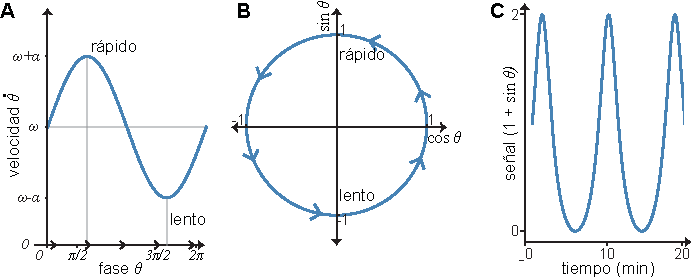
\includegraphics[width=1\columnwidth]{figures/chapter5/C5_determinista_oscilatorio.pdf} 
    \caption{\textbf{Oscilaciones no-uniformes en un modelo de fase con bifurcación de ciclo infinito.} (A) Velocidad de la fase en función de su posición entre $0$ y $2\pi$. El campo de velocidades de $\xx(t)$ también se encuentra indicado con flechas negras sobre el eje $x$. (B) Trayectoria de la fase en la circunferencia trigonométrica. El campo de velocidades de $\xx(t)$ también se encuentra indicado en la circunferencia unitaria con flechas azules. (C) Observable en función del tiempo, definido según la ecuación \ref{C5_eq:seno_fase}. La condición inicial es $\theta(0)= 0$. (A-C) Está representado el caso de oscilaciones no-uniformes de la ecuación \ref{C5_eq:adler_determinista}, donde $\omega > \alpha > 0$. Parámetros: $\omega =2\pi/7 \; \text{min}^{-1}$ y  $\alpha = 0.5 \times 2\pi/7 \; \text{min}^{-1}$. (A,B) Se encuentran indicadas las regiones de máxima y mínima velocidad.}
    \label{C5_fig:adler_determinista_oscilatorio}
\end{figure}


Gracias a la periodicidad del sistema dinámico que estudiamos, otra forma de visualizar su comportamiento es con la circunferencia trigonométrica de radio unidad.\marginpar{circunferencia\\trigonométrica} En esta representación, el eje $x$ corresponde al $\cos{(\theta)}$, el eje $y$ corresponde al $\sin{(\theta)}$, y se dibujan en el plano posibles trayectorias de $\theta(t)$. Por ejemplo, $\theta = 0$ corresponde a las coordenadas $x=1, \; y=0$, ó $\theta = \pi/2$ a $x=0, \; y=1$. Por ende, si $\theta(t)$ toma valores de $0$ a $10\pi$, $\theta(0) = 0$ y su velocidad es positiva y constante, en la circunferencia trigonométrica visualizaremos un círculo de radio uno y el sistema dinámico lo recorrerá en sentido antihorario comenzando en la coordenada $(1,0)$ y con velocidad constante hasta alcanzar la coordenada $(1,0)$ luego de completar $5$ vueltas. En la figura \ref{C5_fig:adler_determinista_oscilatorio}B representamos la circunferencia trigonométrica de radio unidad asociada a la dinámica representada en \ref{C5_fig:adler_determinista_oscilatorio}A. En este caso, la velocidad con que la fase recorre la circunferencia trigonométrica es positiva, pero no es constante, y depende de la localización de la fase $\theta(t)$ en la circunferencia. Las regiones de mayor y menor velocidad de $\theta(t)$ están indicadas, junto con la dirección en que el sistema recorre la circunferencia. 


Pero, ¿cómo potencialmente se relacionaría este sistema dinámico que estamos estudiando con la actividad dinámica de ERK? Previamente establecimos que interpretaríamos un ciclo de la fase $\theta(t)$ como un pulso de actividad de ERK. Entonces, podríamos proponer como observable de la actividad de ERK cualquier función periódica de la fase, de período $2\pi$. De esta manera, la dinámica de activación de ERK estaría gobernada por la fase $\theta(t)$ y este observable representaría la señal de la dinámica de activación de ERK. Esta distinción entre fase y señal explota el hecho de que es más sencillo escribir ecuaciones diferenciales simples que determinen la dinámica del sistema utilizando la variable angular $\theta(t)$ en lugar de cualquiera de sus posibles observables, y que la señal traduce esa dinámica en series temporales que son más fáciles de visualizar e interpretar que la evolución temporal de la fase. A modo ilustrativo, podemos, por ejemplo, proponer representar a la señal adquirida de la actividad dinámica de ERK $s(t)$ como el seno de la fase $\theta(t)$ en función del tiempo. Este observable tiene la ventaja de ser la proyección de la fase $\theta(t)$ en el eje $y$ de la circunferencia trigonométrica. Para trabajar con valores positivos en la señal, proponemos \marginpar{señal de actividad\\de ERK}
\begin{equation}
    s(t) = 1+\sin{\theta(t)}.
    \label{C5_eq:seno_fase}
\end{equation}
Con esta definición, la señal de la dinámica representada en \ref{C5_fig:adler_determinista_oscilatorio}A,B se vería como en la figura \ref{C5_fig:adler_determinista_oscilatorio}C. En esta dinámica, vimos que la velocidad de la fase no era uniforme, y la zona de velocidades más rápidas era la región alrededor de $\pi/2$. En esta zona el seno tiene su máximo, y en la señal $s(t)$ la no-uniformidad se traduce en picos más estrechos comparados con oscilaciones uniformes. Por otro lado, la zona de velocidades más lentas alrededor de $\theta = 3 \pi/2$ conduce a valles más anchos en la señal. 


Hasta ahora, consideramos el sistema dinámico de la ecuación \ref{C5_eq:adler_determinista} para el caso en donde $\alpha$ es positivo y pequeño comparado con $\omega$. Cuando el valor de $\alpha$ se acerca al valor de $\omega$, $\omega - \alpha$ se vuelve cada vez más pequeño, el mínimo del diagrama de fases \ref{C5_fig:adler_determinista_oscilatorio}A se arrima al eje $x$, y la velocidad mínima de la fase $\theta(t)$ se acerca a $0$. En el caso límite donde $\alpha = \omega$, el mínimo del diagrama de fases de \ref{C5_fig:adler_determinista_oscilatorio}A toca al eje $x$, y la velocidad mínima de la fase $\theta(t)$ es $0$. Esto significa que cuando la fase se encuentre en este punto, permanecerá en este punto el resto del tiempo. En otras palabras, el sistema dinámico deja de oscilar en $\theta = 3 \pi/2$.


En el caso donde $\alpha > \omega$, la velocidad de la fase cruza dos veces el eje $x$ en los puntos \xxe y \xxi (figura \ref{C5_fig:adler_determinista_excitable}A). Además, toma valores negativos cuando $\theta$ está comprendido entre \xxe y \xxi. Esto significa que si el sistema se encuentra en cualquier lugar del intervalo $(\xxe,\xxi)$, la fase evolucionará con velocidad negativa hasta llegar a \xxe. De manera equivalente, si el sistema se encuentra en cualquier lugar del intervalo de velocidades positivas $(\xxi,\xxe)$, la fase también evolucionará hasta llegar a \xxe. Por esta característica de sumidero que adquiere \xxe cuando $\alpha > \omega$, se clasifica a \xxe como un punto fijo estable. Representamos al punto fijo estable como un círculo relleno en la figura \ref{C5_fig:adler_determinista_excitable}A. Por el contrario, si el sistema se encuentra en \xxi, el sistema permanecerá en \xxi pues su velocidad es cero. Sin embargo, siempre que el sistema esté inicialmente en cualquier lugar distinto de los puntos fijos, el sistema tiende a escapar de \xxi hacia \xxe. \marginpar{puntos fijos\\estables e\\inestables} Por esta característica de fuente que adquiere \xxi cuando $\alpha > \omega$, donde el sistema tiende a escapar de él, se clasifica a \xxi como un punto fijo inestable. Representamos al punto fijo inestable como un círculo vacío en la figura \ref{C5_fig:adler_determinista_excitable}A.


 \begin{figure}
    \centering
    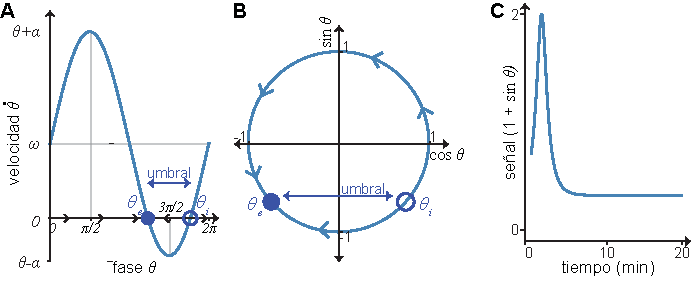
\includegraphics[width=1\columnwidth]{figures/chapter5/C5_determinista_excitable.pdf} 
    \caption{\textbf{Silencios en un modelo de fase con bifurcación de ciclo infinito.} (A) Velocidad de la fase en función de su posición entre $0$ y $2\pi$. El campo de velocidades de $\xx(t)$ también se encuentra indicado con flechas negras sobre el eje $x$. (B) Trayectoria de la fase en la circunferencia trigonométrica. El campo de velocidades de $\xx(t)$ también se encuentra indicado en la circunferencia unitaria con flechas azules. (C) Observable en función del tiempo, definido según la ecuación \ref{C5_eq:seno_fase}. La condición inicial es $\theta(0) = 6$. (A-C) Está representado el caso excitable de la ecuación \ref{C5_eq:adler_determinista}, donde $ 0 < \omega < \alpha$. En este caso, $\omega = 2 \pi/7 \; \text{min}^{-1}$ y $\alpha = 1.1 \times 2 \pi/7 \; \text{min}^{-1}$ y . (A,B) Se encuentran indicados los puntos fijos estable \xxe e inestable \xxi, y el umbral de excitabilidad.}
    \label{C5_fig:adler_determinista_excitable}
\end{figure}


Podemos determinar la localización de los puntos fijos analíticamente calculando dónde la velocidad de fase de la ecuación \ref{C5_eq:adler_determinista} se anula. Sea $\xx_f$ un punto fijo. Por su definición,  
\begin{align}
    &\partial_t \theta (\xx_f) = 0 = \omega + \alpha \sin{\xx_f} \nonumber \\
    &\xx_{f1} = -\arcsin{\frac{\omega}{\alpha}} + 2 n_1 \pi \quad \text{y} \quad
     \xx_{f2} = \pi + \arcsin{\frac{\omega}{\alpha}} + 2 n_2  \pi \quad n_1,n_2 \in \mathbb{Z}. 
    \label{C5_eq:PF_def}
\end{align}
En las figuras \ref{C5_fig:adler_determinista_excitable}A,B están representados los puntos fijos del intervalo $[0,2\pi)$, donde $n_1 = 1$ y $n_2 = 0$. \xxi es el punto fijo inestable, pues 
\begin{align*}
    \frac{d\theta(t)}{dt}|_{\xxi+\epsilon} > 0 \quad \text{y} \quad \frac{d\theta(t)}{dt}|_{\xxi-\epsilon} < 0
\end{align*}
 para $\epsilon$ positivo y pequeño, características de un punto fuente. En cambio, \xxe es el punto fijo estable, pues
 \begin{align*}
    \frac{d\theta(t)}{dt}|_{\xxe+\epsilon} < 0 \quad \text{y} \quad \frac{d\theta(t)}{dt}|_{\xxe-\epsilon} > 0,
\end{align*}
características de sumidero.


Podemos visualizar este régimen dinámico en la circunferencia trigonométrica \ref{C5_fig:adler_determinista_excitable}B. Para cualquier condición inicial en el intervalo $(\xxe,\xxi)$, el sistema recorrerá la circunferencia en sentido horario alejándose de \xxi hasta alcanzar \xxe. En cambio, si la condición inicial del sistema es en $(\xxi,\xxe)$, el sistema recorrerá la circunferencia en sentido antihorario escapando de \xxi hacia \xxe. Ilustramos un ejemplo de la señal que adquiriríamos en este caso en la figura \ref{C5_fig:adler_determinista_excitable}C. La excursión que el sistema dinámico realiza desde su condición inicial hacia el punto fijo estable escapando del inestable se ve en la señal como un pulso transitorio. Luego, cuando el sistema permanece en el punto fijo estable una vez que lo alcanza, se traduce en un silencio en el estacionario de la señal.  


En conclusión, aumentando el valor de $\alpha$ desde $\alpha < \omega$ hacia $\alpha > \omega$ aparecen un punto fijo estable y uno inestable. Esta bifurcación se conoce como bifurcación de \textit{saddle-node} de ciclo infinito\marginpar{bifurcación de\\\textit{saddle-node}\\de ciclo infinito}. Luego, para valores de $\alpha < \omega$, el sistema dinámico de la ecuación \ref{C5_eq:adler_determinista} dará lugar a oscilaciones. Si los ciclos de $\theta$ representaran pulsos de actividad de ERK, los ciclos del régimen oscilatorio representarían oscilaciones de pERK. Cuando $\alpha > \omega$ dará lugar a silencios en el estado estacionario, ya sea luego de realizar una excursión desde su condición inicial hacia el punto fijo estable, o estando inicialmente en cualquiera de los dos puntos fijos. En este caso, este régimen daría lugar a silencios en la dinámica de actividad de ERK. 


Detengámonos, por un momento, en la excursión que puede ocurrir cuando el sistema escapa del punto fijo inestable hacia el estable en el régimen donde $\alpha > \omega$ que da lugar a silencios. Como se puede ver en la figura  \ref{C5_fig:adler_determinista_excitable}C, esta excursión da lugar a un pulso transitorio en la señal. A continuación exploramos la posibilidad de explotar esta propiedad para que en este régimen no sólo sea posible tener silencios, sino también actividad pulsátil a partir de aplicar pequeñas perturbaciones al sistema dinámico que lo muevan de su estado estacionario. 


\section{Excitabilidad en el modelo de fase con bifurcación de ciclo infinito}
\label{C5_sec:perturbacion}

En esta sección queremos evaluar el efecto de aplicar pequeñas perturbaciones al sistema dinámico que describe la ecuación \ref{C5_eq:adler_determinista} en el régimen donde $\alpha > \omega$, y  hay dos puntos fijos. Imaginemos, por ejemplo, que el sistema se encuentra en su estado estacionario en el punto fijo estable \xxe. Dadas sus propiedades de sumidero, si el sistema recibe una pequeña perturbación, rápidamente retornará hacia su estado anterior en \xxe. En la señal, esto se traducirá como una perturbación de baja amplitud (ecuación \ref{C5_eq:seno_fase}). En cambio, si la perturbación es suficientemente grande tal que el sistema es capaz de sobrepasar el punto fijo inestable \xxi, éste realizará una excursión recorriendo gran parte de la circunferencia trigonométrica antes de regresar a su estado anterior en \xxe. En la señal, esto se traducirá como un pulso similar al de la figura \ref{C5_fig:adler_determinista_excitable}C. \marginpar{sistema dinámico\\excitable}Esta característica es propia de sistemas dinámicos excitables. La magnitud de la perturbación, o valor umbral, necesaria para realizar una excursión en el régimen excitable es la distancia angular entre el punto fijo estable y el inestable (figura \ref{C5_fig:adler_determinista_excitable}), es decir,
\begin{align}
    \left| \xxe - \xxi \right| &=  \left| \left(\pi + \arcsin{\frac{\omega}{\alpha}} \right) -  \left(-\arcsin{\frac{\omega}{\alpha}}\right)\right| \\
    &=  \left|\pi + 2 \arcsin{\frac{\omega}{\alpha}}\right|.
    \label{C5_eq:umbral}
\end{align} \marginpar{umbral de\\excitabilidad}
El umbral para realizar una excursión en el régimen excitable depende del cociente adimensional $\omega/\alpha$. Modificando este cociente, es posible modificar el umbral de excitabilidad, y así controlar con qué intensidad deben ser las perturbaciones dar lugar a actividad pulsátil.


En resumen, en presencia de perturbaciones la ecuación \ref{C5_eq:adler_determinista} describe la dinámica de una fase de un sistema dinámico con un régimen excitable cuando $\alpha > \omega$. Cuando la perturbación tiene un valor mayor al umbral de la ecuación \ref{C5_eq:umbral}, el sistema realiza una excursión, y en la serie temporal se visualiza un pulso (ecuación \ref{C5_eq:seno_fase}). Si los ciclos de $\theta$ representaran pulsos de actividad de ERK, una excursión en el régimen excitable representaría un pulso de actividad de ERK, con la posibilidad de ser un pulso aislado entre silencios. Con estas ideas, dado que los pulsos aislados son uno de los elementos dinámicos característicos de las oscilaciones intermitentes de actividad de ERK, en la próxima sección proponemos incorporar al modelo teórico la posibilidad de tener perturbaciones de manera sistemática.  


\section{El ruido blanco gaussiano aditivo induce una dinámica pulsátil en el régimen excitable }
\sectionmark{El ruido blanco gaussiano aditivo induce una dinámica pulsátil...}
\label{C6_sec:alder_ruido}

Proponemos introducir perturbaciones al modelo de fase con bifurcación de ciclo infinito de la ecuación \ref{C5_eq:adler_determinista} a partir de agregar ruido blanco gaussiano aditivo \cite{Lindner2004}
\begin{equation}
    \dot{\theta}(t) = \omega + \alpha \sin{(\theta(t))} + \sqrt{2D} \xi_w(t).
    \label{C6_eq:adler_white_noise}
\end{equation}
\marginpar{ruido blanco\\gaussiano}
La primera parte de esta ecuación es la ecuación de Adler con la que trabajamos previamente, y el último término describe el ruido blanco gaussiano. Intuitivamente, el ruido blanco representa un proceso que en cada instante de tiempo adquiere un valor finito que es independiente al valor que tomó en el instante de tiempo anterior, cuyo valor medio a lo largo del tiempo es cero y su varianza, constante. Esto implica que en el perfil de frecuencias de la señal, la contribución del ruido es de igual amplitud para todas las frecuencias. Que sea gaussiano significa que los valores que toma el proceso en cada instante de tiempo están sampleados de una distribución gaussiana de media cero y varianza constante $D$. Formalizando, la variable $\xi_w(t)$ de la ecuación diferencial estocástica \ref{C6_eq:adler_white_noise} representa un proceso de ruido blanco gaussiano derivado de un proceso de Wiener, tal que \cite{SanMiguel2000}
\begin{align}
    \langle \xi_w(t) \rangle_{t} & = 0 \label{C6_eq:wiener_mean}\\
    \langle \xi_w(t),\xi_w(t') \rangle_{t} & = \delta_{t,t'}. \label{C6_eq:wiener_cov}
\end{align}



La ecuación \ref{C6_eq:adler_white_noise} cuenta ahora con tres parámetros: la frecuencia del caso uniforme $\omega$, la amplitud de modulación $\alpha$, y la \textbf{intensidad del ruido} $D$,\marginpar{intensidad del ruido} que tiene unidades de $\text{tiempo}^{-2}$. Esta ecuación diferencial consiste en una parte determinista, que estudiamos en las secciones anteriores, y una parte estocástica, el ruido blanco gaussiano aditivo de intensidad $D$. Con este nuevo término, en cada instante de tiempo la fase $\xx(t)$ recibe una perturbación de cierta magnitud. Esta magnitud está sampleada de una distribución gaussiana cuya varianza es $D$. Entonces, cuanto más grande es la intensidad del ruido, la probabilidad de tener perturbaciones más grandes y que eventualmente conduzcan a la aparición de pulsos en el régimen excitable aumenta.  


Antes de continuar, es necesario hacer una breve aclaración técnica. Dependiendo de la definición del ruido, el proceso resultante de ecuaciones estocásticas de la forma de \ref{C6_eq:adler_white_noise} puede ser una función no continua en el tiempo. Cuando esto ocurre, se produce una ambigüedad en algunas expresiones matemáticas, que se resuelve fácilmente definiendo una única interpretación. En este trabajo utilizaremos la interpretación de Itô \cite{SanMiguel2000}. 



En la figura \ref{C6_fig:traces} observamos series temporales del observable \ref{C5_eq:seno_fase}, donde la dinámica de la fase $\xx(t)$ está determinada por la ecuación \ref{C6_eq:adler_white_noise}. Tanto para el caso donde las oscilaciones son uniformes y $\dddelta = 0$, como para el caso de oscilaciones no-uniformes donde $1 > \dddelta > 0$, a medida que crece la intensidad del ruido las oscilaciones van perdiendo su regularidad, hasta que la dinámica parece ser directamente gobernada por el ruido para valores altos de $D$. En el régimen donde $\dddelta >1$, no observamos dinámica para valores de ruido pequeños, similar a las observaciones de la sección \ref{C5_sec:osc_exc}. Para valores intermedios de ruido, observamos actividad pulsátil en el régimen excitable. Una interpretación posible es que el sistema inicialmente se encuentra en el punto fijo estable \xxe de la figura \ref{C5_fig:adler_determinista_excitable}A, B. El ruido perturba al sistema de esa posición, y el sistema fluctúa alrededor del punto fijo estable. En un dado momento, la perturbación del ruido tiene la fuerza necesaria para que el sistema sobrepase el punto fijo inestable \xxi, dando lugar a una excursión desde ese lugar hasta el punto fijo estable siguiente. Esa excursión se ve como un pulso en la señal $s(t)$. Para un mismo valor de \dddelta observamos que la actividad pulsátil es cada vez más frecuente  a medida que crece el ruido. Cuando aumenta la intensidad $D$ del ruido, los valores que éste puede tomar en cada instante de tiempo tienen mayor probabilidad de ser más grandes. A medida que aumenta el ruido es más probable que el sistema atraviese el punto fijo inestable en el mismo intervalo de tiempo. En los casos en donde la intensidad del ruido toma valores altos, la dinámica parece ser completamente gobernada por el ruido, y a simple vista indistinguible de series temporales del régimen oscilatorio para los mismos valores de $D$. Por otro lado, para valores intermedios y fijos de ruido, la dinámica pulsátil es menos frecuente en el régimen excitable a medida que crece \dddelta. Observamos previamente que el umbral que determina la magnitud de la perturbación ante la que ocurre un pulso depende del cociente \dddelta (ecuación \ref{C5_eq:umbral}). Luego, a medida que el cociente \dddelta crece, para atravesar el umbral es necesario perturbaciones más grandes del sistema, que son más probables con valores más grandes de $D$.

 \begin{figure}
    \centering
    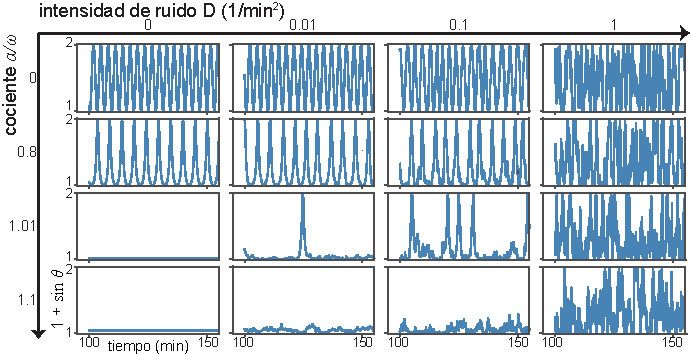
\includegraphics[width=1\columnwidth]{figures/chapter6/C6_traces.pdf} 
    \caption{\textbf{Actividad pulsátil en el régimen excitable del modelo de fase con bifurcación de ciclo infinito y ruido blanco gaussiano aditivo.} Series temporales que representan la dinámica de la fase gobernada por la ecuación \ref{C6_eq:adler_white_noise}, en donde el observable es \ref{C5_eq:seno_fase}. De arriba hacia abajo, la primera fila representa el caso oscilatorio uniforme. La segunda fila representa el caso de oscilaciones no-uniformes, y las dos filas restantes son casos excitables. Las series temporales fueron obtenidas a partir de simulaciones descriptas en el apéndice \ref{C6_ap:traces}, donde la frecuencia del caso oscilatorio uniforme $\omega = 18\pi/28 \; \text{min}^{-1}$, la frecuencia de sampleo $dt$ fue de $10^{-4}$, la frecuencia de adquisición $d$ fue de $10$, el total de tiempo de la simulación $T$ fue de $1000$ minutos. Las condiciones iniciales fueron sampleadas de una distribución uniforme $U(0,2\pi)$. Las series temporales fueron graficadas desde los $100$ minutos para evitar visualizar efectos transitorios.}
    \label{C6_fig:traces} 
\end{figure}



En definitiva, el ruido promueve la aparición de pulsos en el régimen excitable, y la tasa de pulsado aumenta, al menos cualitativamente, conforme a la intensidad del ruido. A diferencia del régimen oscilatorio, en este régimen no hay una estructura temporal periódica subyacente que los ordene. Sin embargo, en principio, la dinámica pulsátil podría tener una estructura dinámica alternativa que ordene los pulsos, y evaluamos esta posibilidad. Para estudiar estructuras dinámicas en series temporales pulsátiles, es común utilizar observables basados en el espectro de potencias de Fourier, ya que tienen un significado intuitivo inmediato y son fácilmente medibles en series temporales obtenidas a partir de simulaciones \cite{Gammaitoni1998}. Definimos el espectro de consenso de las series temporales $s(t)$ como \cite{Ditzinger1994} \marginpar{espectro de consenso}
\begin{equation}
    \langle S_k \rangle = \frac{1}{N} \sum_{i=1}^N |A_k|^2,
    \label{C6_eq:espectro_consenso}
\end{equation}
donde $A_k$ es el espectro de amplitud de Fourier definido según \ref{C2_eq:amplitud_fourier}, y $N$ es la cantidad de series temporales consideradas. En la figura \ref{C6_fig:SR}A graficamos el espectro de consenso de series temporales adquiridas en el régimen excitable. Para valores bajos de intensidad de ruido, el espectro de consenso muestra un pequeño máximo en frecuencias bajas. La altura del máximo del espectro y su frecuencia fundamental aumentan con la intensidad del ruido $D$. Tras un valor umbral de intensidad de ruido, la altura del pico del espectro y la frecuencia fundamental comienzan a disminuir. Finalmente, para un $D$ suficientemente grande, la frecuencia fundamental se desplaza a cero, efecto característico de las dinámicas completamente dominadas por el ruido. Este comportamiento del espectro de consenso en función del ruido sugiere la presencia de una dinámica pulsátil coherente estimulada por el ruido, en donde la coherencia está optimizada en valores intermedios de $D$. 


 \begin{figure}
    \centering
    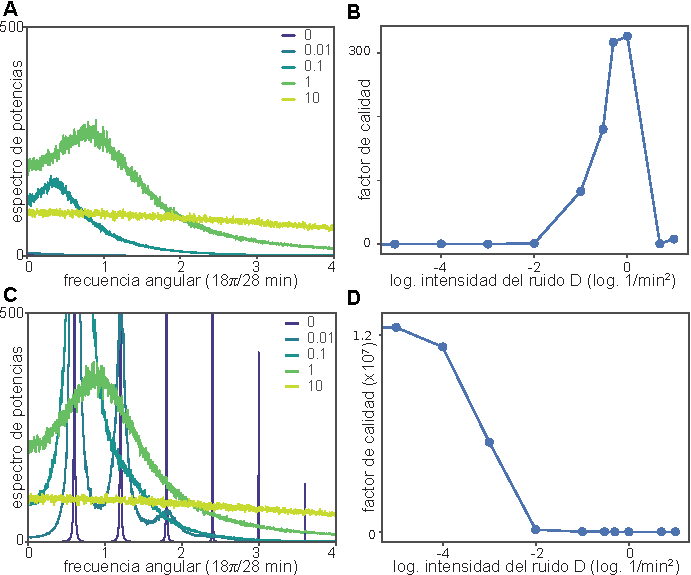
\includegraphics[width=1\columnwidth]{figures/chapter6/C6_SR.pdf} 
    \caption{\textbf{Resonancia estocástica en el régimen excitable del modelo de fase con bifurcación infinita y ruido blanco aditivo.} (A) Espectro de consenso de para el caso excitable del modelo de fase de bifurcación de ciclo infinito con ruido blanco gaussiano aditivo (ecuación \ref{C6_eq:espectro_consenso}). $\omega = 18\pi/28 \; \text{min}^{-1}$ y $\dddelta = 1.1$. (B) Factor de calidad en función de la intensidad del ruido, calculado a partir de los datos de A (ecuación \ref{C6_eq:QF}). (C) Espectro de consenso para el caso oscilatorio no-uniforme del modelo de fase de bifurcación de ciclo infinito con ruido blanco gaussiano aditivo. $\omega = 18\pi/28 \; \text{min}^{-1}$ y $\dddelta = 0.8$. (D) Factor de calidad en función de la intensidad del ruido, calculado a partir de los datos de C. (A-D)  $N=500$ series temporales simuladas (apéndice \ref{C6_ap:traces}). La frecuencia de sampleo $dt$ fue de $10^{-4}$, la frecuencia de adquisición $d$ fue de $10$, el total de tiempo de la simulación $T$ fue de $1000$ minutos, y las condiciones iniciales fueron sampleadas de una distribución uniforme $U(0,2\pi)$. (A,C) La intensidad del ruido está indicada en escala de colores.}
    \label{C6_fig:SR}
\end{figure}


Para formalizar esta interpretación, podemos usar del factor de calidad, un parámetro adimensional que cuantifica el rendimiento de un oscilador o resonador. Formalmente, definimos el factor de calidad $\beta$ como \cite{Ditzinger1994} \marginpar{factor de calidad}
\begin{equation} 
    \beta = \omega_0 \frac{\langle S_0 \rangle}{\Delta  \omega_0},
    \label{C6_eq:QF}
\end{equation}
donde $\langle S_0 \rangle$ es la amplitud del espectro de consenso de la señal $s(t)$ en su frecuencia fundamental $\omega_0$. $\Delta  \omega_0$ es una medida del ancho del espectro de consenso en su frecuencia fundamental, definido como el ancho del espectro cuando su altura es $\langle S_0 \rangle / \sqrt{e}$. Con esta definición, el factor de calidad es grande cuando el ancho del espectro de consenso es pequeño, es decir, cuando adquirimos señales puras del sistema.  El factor $\omega_0$ de esta definición determina que el factor de calidad será mayor a frecuencias mayores, frecuencias que se alejan del ruido blanco. En la figura  \ref{C6_fig:SR}B podemos observar el factor de calidad correspondiente a los datos de la figura \ref{C6_fig:SR}A. Observamos que $\beta$ aumenta conforme a la intensidad del ruido, manifestando una dinámica cada vez más coherente. Luego de alcanzar un máximo, la curva del factor de calidad decrece, retratando que el ruido destruye gradualmente el movimiento coherente. El máximo revela la existencia de un ruido óptimo que produce la dinámica más coherente dentro del régimen excitable. Este efecto es propio de sistemas de resonancia estocástica.\marginpar{resonancia\\estocástica}


En las figuras \ref{C6_fig:SR}C, D mostramos el espectro de consenso y el factor de calidad para el caso de oscilaciones no-uniformes. Para valores bajos de ruido, donde domina el comportamiento determinista, el espectro de frecuencias consiste en una frecuencia fundamental bien definida, y frecuencias secundarias que reflejan la no-uniformidad de la señal. A medida que aumenta la intensidad del ruido, el pico del espectro se va ensanchando y corriendo hacia frecuencias fundamentales más grandes y el factor de calidad decrece. Esto indica que el ruido destruye gradualmente el movimiento coherente determinista. Si la intensidad del ruido es lo suficientemente grande, el espectro de Fourier indica que el movimiento está completamente dominado por el ruido. 


En definitiva, agregar ruido blanco gaussiano aditivo al modelo de fase de bifurcación de ciclo infinito da lugar a actividad pulsátil en el régimen excitable. Además, el ruido regula la coherencia de la actividad pulsátil en el régimen excitable, y la desordena en el régimen oscilatorio. De esta manera, este modelo tiene la posibilidad de generar los principales elementos dinámicos que caracterizamos en las oscilaciones intermitentes, es decir, intervalos oscilatorios, de silencio y pulsos aislados. A partir de estas observaciones, se abre la pregunta de si es posible explotar sus propiedades o combinar estos elementos dinámicos para lograr reproducir nuestras observaciones de la dinámica de actividad de ERK en un modelo con la menor cantidad de parámetros posible. La resonancia estocástica que observamos en el régimen excitable nos conduce a preguntarnos si perturbando de manera sistemática al sistema en el régimen excitable es posible reproducir las transiciones entre intervalos oscilatorios o trenes de pulsos coherentes, silencios y pulsos aislados. Alternativamente, las oscilaciones intermitentes podrían ser descriptas como oscilaciones desordenadas. Como otra posibilidad, podrían ser descriptas como transiciones entre el estado excitable y el oscilatorio. 


En el modelo conceptual que construimos de la dinámica de activación de ERK en ESCs, proponemos que las oscilaciones están controladas por la dosis de FGF4, que además controla la duración de los intervalos oscilatorios. A pesar de que la duración de los intervalos aumente con la dosis de estímulo, el valor modal de la duración de pulsos parece conservarse. Luego, analizar cómo depende la duración de pulsos de los parámetros del modelo con el que proponemos comenzar a trabajar contribuirá a proponer y evaluar posibles descripciones de las oscilaciones intermitentes.

%Además, en el modelo de fase con bifurcación de ciclo infinito y ruido blanco gaussiano, la expresión analítica de la duración de pulsos es desconocida. Al ser éste un modelo utilizado también para describir muchos otros fenómenos de la física y la biología, calcularla significa una contribución importante de por sí al área de procesos estocásticos. 

\section{La duración de pulsos diverge en la bifurcación en ausencia de ruido}
\sectionmark{Sin ruido la duración de pulsos diverge en la bifurcación}

Para entender cómo se comporta la duración de pulsos ante la variación de los parámetros del modelo, comenzamos por trabajar con el modelo determinista \ref{C5_eq:adler_determinista}. Primero mostramos cómo calcular la expresión analítica de la duración de pulsos en el régimen oscilatorio donde $\alpha < \omega$, resultado previamente conocido \cite{Strogatz1994}. Luego, proponemos una definición de duración de pulsos para el régimen excitable, definición que será importante para el resto del trabajo. A partir de esta definición, obtenemos una expresión para la duración de pulsos en este régimen, donde $\alpha > \omega$ y consideramos una pequeña perturbación.


\subsection{Duración de pulsos en el régimen oscilatorio }
\label{C5_sec:T_osc}
%Luego, obtenemos una expresión para el régimen excitable, en donde consideramos una pequeña perturbación en el modelo determinista. Finalmente, calculamos la duración de pulsos en el modelo con ruido blanco gaussiano aditivo. 

En un sistema dinámico oscilatorio, la duración de pulsos se corresponde con el período de oscilación $T_{\text{osc}}$ 
\begin{align}
    T_{\text{osc}}&= \int dt \nonumber \\ 
    &= \int_{0}^{2 \pi} \frac{dt}{d\theta} d\theta \nonumber \\
    &= \int_{0}^{2 \pi} \frac{1}{\omega + \alpha \sin{\theta}} d\theta.
    \label{C5_eq:T_osc_def}
\end{align}
Para resolver esta integral, proponemos el cambio de variables $z = e^{i \theta}$, donde 
\begin{align}
    d\theta = \frac{1}{iz} dz \quad \text{y} \quad \sin{\theta} = \frac{z - \overline{z}}{2} = \frac{z^{2} - 1}{2} \cdot \frac{1}{z},
\end{align}
e integraremos en la circunferencia de radio unidad centrada en cero $C_{0,1}$. Luego, la expresión \ref{C5_eq:T_osc_def} queda como
\begin{align}
    T_{\text{osc}}&= \int_{0}^{2 \pi} \frac{1}{\omega + \alpha \sin{\theta}} d\theta \nonumber \\
    &= \frac{2}{\alpha} \oint_{C_{0,1}} \frac{1}{2 \frac{\omega}{\alpha} + \frac{z^{2} - 1}{z}} \; \frac{dz}{iz} \nonumber\\
    &= \frac{2}{i \alpha} \oint_{C_{0,1}} \frac{1}{2 \frac{z}{\delta} + z^{2}-1}dz,
    \label{C5_eq:T_osc_cambio_variables}
\end{align}
 donde definimos la variable adimensional $\delta = \dddelta$. Para factorizar el denominador, es conveniente buscar sus ceros $z_\pm$
\begin{align}
    z_\pm^{2} + 2 \frac{z_\pm}{\delta} - 1=0 \nonumber\\
    z_\pm = -\frac{1}{\delta}  \pm \kappa
\end{align}
donde definimos $\kappa = \sqrt{1/\delta^{2} + 1}$. Con este resultado, es posible factorizar el denominador de la expresión \ref{C5_eq:T_osc_cambio_variables}, tal que 
\begin{equation}
    T_{\text{osc}}= \frac{2}{i \alpha} \oint_{C_{0,1}} \frac{1}{z-( -\frac{1}{\delta} + \kappa)} \; \frac{1}{z + (\frac{1}{\delta} + \kappa)} dz.
    \label{C5_eq:T_osc_factorizada}
\end{equation}
Para resolver la integral, utilizaremos el Teorema de los residuos. Para implementar este teorema, es necesario primero localizar los polos, es decir, los valores de $z$ que anulan el denominador. Para el régimen oscilatorio de la ecuación \ref{C5_eq:adler_determinista}, $\omega > \alpha $. Esta relación implica que $1/\delta >1$, y el polo correspondiente a $z_- = -1/\delta  - \kappa $ está fuera de la circunferencia $C_{0,1}$. En cambio, $\kappa - 1/\delta < 1 $ y el polo correspondiente a $z_+$ se encuentra dentro de $C_{0,1}$. Esto demuestra que existe una sola singularidad aislada dentro de la región de integración, la circunferencia unitaria. El corolario del Teorema de Cauchy nos asegura que esta integral existe, y el Teorema de los residuos nos conduce al siguiente resultado \cite{Strogatz1994}

\begin{align}
   T_{\text{osc}} &= \frac{2}{i\alpha} 2\pi i \lim_{z \to -\frac{1}{\delta} + \kappa} \frac{z-(-\frac{1}{\delta} + \kappa)}{[z-(-\frac{1}{\delta} + \kappa)][z + (\frac{1}{\delta} + \kappa)] } \nonumber\\
    &= \frac{4\pi}{\alpha} \lim_{z \to -\frac{1}{\delta} + \kappa} \frac{1}{z + (\frac{1}{\delta} + \kappa)} \nonumber \\
     &= \frac{4\pi}{\alpha}  \frac{1}{\frac{-1}{\delta} + \kappa + \frac{1}{\delta} + \kappa} \nonumber \\
     &=\frac{4\pi}{\alpha}  \frac{1}{2 \kappa} \nonumber\\
     &= \frac{2\pi}{\alpha \sqrt{\frac{1}{\delta^{2}} + 1}} \nonumber \\
       T_{\text{osc}} &= \frac{2\pi}{\sqrt{\omega^{2}-\alpha^{2}}}.
      \label{C5_eq:T_osc}
\end{align}
Es decir, para el sistema dinámico descripto por la ecuación de Adler la duración de pulsos en el régimen oscilatorio depende de sus dos parámetros $\alpha$ y $\omega$. Para independizarnos de la escala temporal, podemos escribir a $T_{\text{osc}}$ como
\begin{align}
    T_{\text{osc}} &= \frac{2\pi}{\omega} \times \frac{1}{\sqrt{1-\frac{\alpha^{2}}{\omega^{2}}}}.
\end{align}
El primer factor de esta expresión es el resultado para el oscilador uniforme, que se recupera cuando $\alpha = 0$. El segundo factor tiene origen en la no-homogeneidad del sistema. En la figura \ref{C5_fig:T_osc} representamos la duración de pulsos en función del cociente entre la amplitud de modulación y la frecuencia del uniforme \dddelta para distintos valores de $\omega$. Observamos que la duración de pulsos aumenta conforme al aumento de \dddelta, y aumenta cuando disminuye la frecuencia del uniforme para valores fijos del cociente \dddelta. Este comportamiento evidencia que cuanto más aumenta la diferencia entre la frecuencia del uniforme y la amplitud de modulación (ya sea disminuyendo $\omega$ y manteniendo \dddelta fijo, o aumentando \dddelta con $\omega$ fijo), el sistema es cada vez menos uniforme y la duración de pulsos se vuelve más larga. Una interpretación posible es que a medida que disminuye la velocidad mínima y aumenta la velocidad máxima de la fase, el sistema pasa cada vez más tiempo en la región de velocidades mínimas, y menos en la de velocidades máximas (figura \ref{C5_fig:adler_determinista_oscilatorio}). Este comportamiento conduce a un aumento en la duración de los pulsos \cite{Strogatz1994}. En los casos límites, cuando \dddelta se anula se recupera el resultado del oscilador uniforme, y en el límite donde $\alpha = \omega$ -cuando se produce la bifurcación de \textit{saddle-node} de ciclo infinito- la duración de pulsos es infinita. %A continuación, queremos estudiar si esta tendencia se conserva en el régimen excitable. 


 \begin{figure}
    \centering
    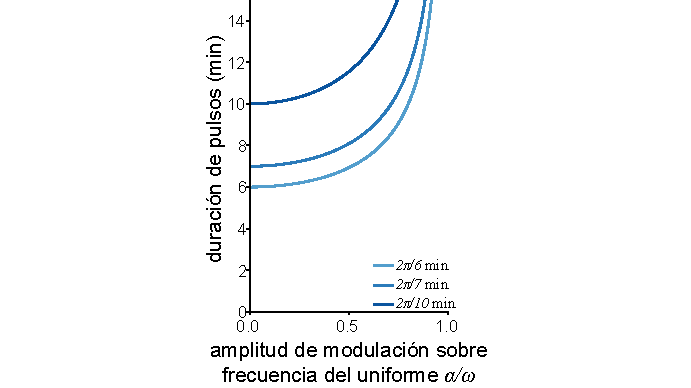
\includegraphics[width=1\columnwidth]{figures/chapter5/C5_T_osc.pdf} 
    \caption{\textbf{La duración de pulsos aumenta cuando el sistema se acerca de la bifurcación en el régimen oscilatorio sin ruido.} Duración de pulsos del sistema dinámico determinista \ref{C5_eq:adler_determinista}. Se observa su comportamiento en función del cociente entre la amplitud de modulación y la frecuencia del uniforme \dddelta, para los valores de $\omega$ indicados.}
    \label{C5_fig:T_osc}
\end{figure}


\subsection{Duración de pulsos en el régimen excitable}
\label{C5_sec:T_exc}

En el régimen excitable de \ref{C5_eq:adler_determinista}, donde $\alpha > \omega$, hay un punto fijo inestable \xxi y un punto fijo estable \xxe, y el sistema tiende a permanecer en \xxe (figura \ref{C5_fig:adler_determinista_excitable}). Un ciclo de la fase \xx se consigue aplicando al sistema una perturbación mayor al umbral de excitabilidad, donde la fase sobrepasará el punto fijo inestable y hará una excursión antes de regresar al punto fijo estable (sección \ref{C5_sec:perturbacion}, ecuación \ref{C5_eq:umbral}). Esta excursión se traduce en un pulso de la señal $s(t)$ (ecuación \ref{C5_eq:seno_fase}). Entonces, formalmente definimos un \textbf{pulso en el régimen excitable} cuando el sistema sobrepasa \xxi y realiza una excursión hacia el punto fijo estable siguiente \xxe.\marginpar{duración de pulsos en el régimen excitable} La \textbf{duración de un pulso en el régimen excitable} $T_{\text{exc}}$ es, entonces, el tiempo que tarda el sistema en llegar a \xxe, habiendo partido de \xxi. Analíticamente, proponemos una definición análoga a la expresión \ref{C5_eq:T_osc_def}, 
\begin{align}
    T_{\text{exc}} = \int_{\xxi}^{\xxe}  \frac{1}{\omega + \alpha \sin{\xx}} d\xx. \label{C5_eq:T_exc_def}
\end{align}
En este caso, en lugar de integrar a lo largo de todo el círculo como hicimos en el caso del régimen oscilatorio, fijamos los límites de integración en el punto fijo inestable \xxi y el punto fijo estable siguiente \xxe. Por simplicidad, elegimos $n_1,n_2 = 0$ en la definición \ref{C5_eq:PF_def}, y los límites de integración son
\begin{equation}
    \xxi = -\arcsin{\frac{\omega}{\alpha}} \quad \xxe = \pi + \arcsin{\frac{\omega}{\alpha}} \quad \text{para } \xxi,\xxe \in [-\frac{\pi}{2},\frac{3\pi}{2}).
\end{equation}
La región de integración está representada en la circunferencia trigonométrica de la figura \ref{C5_fig:T_exc_def}A. 


 \begin{figure}
    \centering
    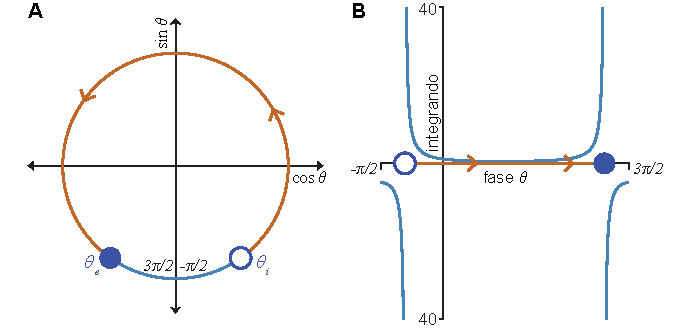
\includegraphics[width=1\columnwidth]{figures/chapter5/C5_T_exc_def.pdf} 
    \caption{\textbf{Duración de pulsos en el régimen excitable.} (A) Trayectoria de la variable de integración en la circunferencia trigonométrica (azul). (B) Integrando de \ref{C5_eq:T_exc_def} en función de su variable de integración. (A,B) Se encuentran indicados los puntos fijos estable \xxe (círculo azul relleno) e inestable \xxi (círculo azul vacío). El intervalo de integración de la definición \ref{C5_eq:T_exc_def} está representando en naranja, y  las flechas naranjas indican la dirección de integración. Los límites del dominio del intervalo de integración están indicados. Parámetros: $\omega=2\pi/7\;\text{min}^{-1}$, $\alpha = 1.1 \times 2\pi/7\;\text{min}^{-1}$.}
    \label{C5_fig:T_exc_def}
\end{figure}


Por su definición formalizada en \ref{C5_eq:PF_def}, el denominador del integrando de \ref{C5_eq:T_exc_def} se anula en los puntos fijos. Esta propiedad conduce a que el integrando diverja en los límites de integración, y en consecuencia que diverja la integral \ref{C5_eq:T_exc_def} (figura \ref{C5_fig:T_exc_def}B). Este resultado es consecuencia de que, sin perturbación, el sistema tarda infinito tiempo en salir del punto fijo inestable. Proponemos salvar esta divergencia realizando la integral \ref{C5_eq:T_exc_def} en un entorno de los puntos fijos. De esta manera, explicitamos en el cálculo la perturbación que el sistema recibe es mayor al umbral de excitabilidad, tal que
\begin{align}
    T_{\text{exc}} = \int_{\xxi+\epsilon_\theta}^{\xxe-\epsilon_\theta}  \frac{1}{\omega + \alpha \sin{\xx}} d\xx \qquad \text{con } 0<\epsilon_\theta \ll 1.
    \label{C5_eq:T_exc_def_eps}
\end{align}


%Esta propuesta está representada en la figura PONER FIGURA. 
%VER SI LA CONVERGENCIA AL PUNTO FIJO ESTABLE ES ASINTOTICA O NO


Es útil reescribir la integral \ref{C5_eq:T_exc_def_eps} para obtener una expresión más sencilla de integrar. Primero efectuamos una traslación de la variable de integración \xx
\begin{align}
    \xx &= \gamma + \frac{\pi}{2} \qquad 
    d\xx = d\gamma. 
\end{align}
Con esta operación, trasladamos a los puntos fijos desde los cuadrantes $[-\pi/2,3\pi/2)$ hacia $[-\pi, \pi)$. Los puntos fijos quedan simétricos respecto del cero (figura \ref{C5_fig:T_exc_T1}A), con valores
\begin{align}
    \gamma_i &= -\arcsin{\frac{\omega}{\alpha}} - \frac{\pi}{2} \qquad
    \gamma_e = \arcsin{\frac{\omega}{\alpha}} + \frac{\pi}{2}.
\end{align}
La integral \ref{C5_eq:T_exc_def_eps} queda escrita como (figura \ref{C5_fig:T_exc_T1}B)
\begin{align}
    T_{\text{exc}} = \int_{\gamma_i+\epsilon_\gamma}^{\gamma_e-\epsilon_\gamma}  \frac{1}{\omega + \alpha \cos{\gamma}} d\gamma \qquad \text{con } 0 < \epsilon_\gamma \ll 1.
    \label{C5_eq:T_exc_def_T1}
\end{align}

 \begin{figure}
    \centering
    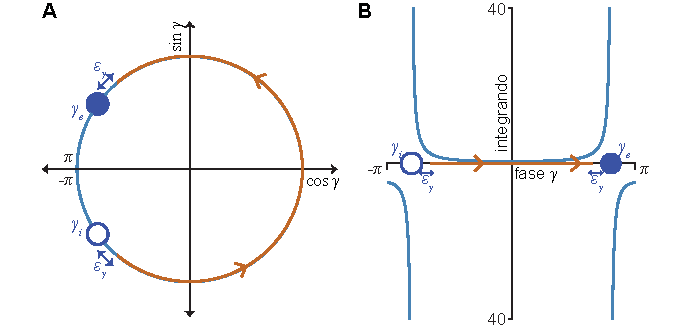
\includegraphics[width=1\columnwidth]{figures/chapter5/C5_T_exc_T1.pdf} 
    \caption{\textbf{Paso intermedio en el cómputo de la duración de pulsos para el régimen excitable.} (A) Trayectoria de la variable de integración en la circunferencia trigonométrica (azul). (B) Integrando de \ref{C5_eq:T_exc_def_T1} en función de su variable de integración. (A,B). Se encuentran indicados los puntos fijos estable \xxe (círculo azul relleno) e inestable \xxi (círculo azul vacío). El intervalo de integración está representando en naranja, y  las flechas naranjas indican la dirección de integración. A modo cualitativo, se indica $\epsilon_\gamma$. Se incluyen también los límites del dominio del intervalo de integración. Parámetros: $\omega=2\pi/7\;\text{min}^{-1}$, $\alpha = 1.1 \times 2\pi/7\;\text{min}^{-1}$.}
    \label{C5_fig:T_exc_T1}
\end{figure}

A continuación, realizamos la siguiente transformación de la variable de integración $\gamma$
\begin{align}
    \beta &= \frac{\gamma}{2} \qquad
    d\beta = \frac{d\gamma}{2}.
    \label{C5_eq:T_exc_T2}
\end{align}
Los valores de $\gamma$ se encuentran en el intervalo $[\gamma_i,\gamma_e] \in [-\pi, \pi)$. La transformación \ref{C5_eq:T_exc_T2} posiciona a los puntos fijos dentro del intervalo $[-\pi/2,\pi/2)$ (figura \ref{C5_fig:T_exc_T2}A), tal que
\begin{align}
    \gamma_i &= - \frac{1}{2} \arcsin{\frac{\omega}{\alpha}} - \frac{\pi}{4} \qquad
    \gamma_e  = \frac{1}{2} \arcsin{\frac{\omega}{\alpha}} + \frac{\pi}{4}.
\end{align}
La integral \ref{C5_eq:T_exc_def_T1} queda expresada como (figura \ref{C5_fig:T_exc_T2}B)
\begin{align}
    T_{\text{exc}} = \int_{\beta_i+\epsilon_\beta}^{\beta_e-\epsilon_\beta}  \frac{2}{\omega + \alpha \cos{2 \beta}} d\beta \qquad \text{con } 0< \epsilon_\beta \ll 1.
    \label{C5_eq:T_exc_def_T2}
\end{align}

 \begin{figure}
    \centering
    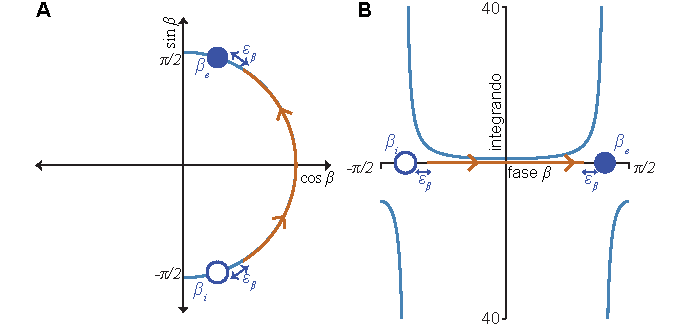
\includegraphics[width=1\columnwidth]{figures/chapter5/C5_T_exc_T2.pdf} 
    \caption{\textbf{Paso intermedio en el cómputo de la duración de pulsos para el régimen excitable.} (A) Trayectoria de la variable de integración en la circunferencia trigonométrica (azul). (B) Integrando de \ref{C5_eq:T_exc_def_T2} en función de su variable de integración. (A,B) Se encuentran indicados los puntos fijos estable \xxe (círculo azul relleno) e inestable \xxi (círculo azul vacío). El intervalo de integración está representando en naranja, y  las flechas naranjas indican la dirección de integración. A modo cualitativo, se indica $\epsilon_\beta$. Se incluyen también los límites del dominio del intervalo de integración. Parámetros: $\omega=2\pi/7\;\text{min}^{-1}$, $\alpha = 1.1 \times 2\pi/7\;\text{min}^{-1}$.}
    \label{C5_fig:T_exc_T2}
\end{figure}

Para terminar, transformamos la variable $\beta$ como
\begin{align}
    \lambda &= \tan{\beta} \qquad
    d\lambda = (1+\lambda^2) d\beta. 
    \label{C5_eq:T_exc_T3}
\end{align}
En el intervalo $[-\pi/2,\pi/2)$ donde está contenida la región de integración definida para $\beta$, la función tangente es biyectiva, lo que permite realizar el cambio de variables \ref{C5_eq:T_exc_T3}. Además es creciente, y el subespacio $[-\pi/2,0)$ mapea a números negativos de $\lambda$, y $(0,\pi/2]$ a positivos. Ahora es necesario reescribir la integral \ref{C5_eq:T_exc_def_T2} en función de la nueva variable $\lambda$. Para reescribir el denominador, resultan útiles las relaciones trigonométricas
\begin{align}
    \cos{\beta} = \frac{1}{\sqrt{1+\lambda^2}} \quad \text{y} \quad \sin{\beta} = \frac{\lambda}{\sqrt{1+\lambda^2}}.
\end{align}
Luego,
\begin{align}
    \cos{2 \beta} &= \cos^2(\beta)-\sin^2(\beta) \nonumber\\
    &=\frac{1}{1+\lambda^2} -  \frac{\lambda^2}{1+\lambda^2} \nonumber\\
    &= \frac{1-\lambda^2}{1+\lambda^2}.
\end{align}
Si incorporamos estas expresiones, la duración de pulsos queda expresada como
\begin{align}
    T_{\text{exc}} &= \int_{\lambda_i+\epsilon}^{\lambda_e -\epsilon} \frac{1}{\omega + \alpha \frac{1-\lambda^2}{1+\lambda^2}} \; \frac{2}{1+\lambda^2} d\lambda \nonumber\\
    &= \frac{2}{\omega}\int_{\lambda_i+\epsilon}^{\lambda_e -\epsilon} d\lambda \frac{1}{1+\lambda^2+\ddelta \left(1-\lambda^2 \right)} \nonumber\\
    &= \frac{2}{\omega}\int_{\lambda_i+\epsilon}^{\lambda_e -\epsilon} d\lambda \frac{1}{\left(1+\ddelta \right) + \left( 1-\ddelta\right) \lambda^2} \qquad \text{con } 0<\epsilon \ll 1. \label{C5_eq:T_exc_def_T3}
\end{align}

 \begin{figure}
    \centering
    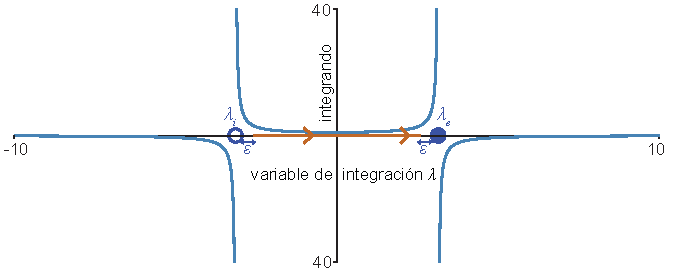
\includegraphics[width=1\columnwidth]{figures/chapter5/C5_T_exc_T3.pdf} 
    \caption{\textbf{Paso intermedio en el cómputo de la duración de pulsos para el régimen excitable.} Integrando de \ref{C5_eq:T_exc_def_T3} en función de su variable de integración. Se indican los puntos fijos estable \xxe (círculo azul relleno) e inestable \xxi (círculo azul vacío). El intervalo de integración está representando en naranja, y  las flechas naranjas indican la dirección de integración. A modo cualitativo, se indica $\epsilon$. Parámetros: $\omega=2\pi/7\;\text{min}^{-1}$, $\alpha = 1.1 \times 2\pi/7\;\text{min}^{-1}$.}
    \label{C5_fig:T_exc_T3}
\end{figure}

La integral \ref{C5_eq:T_exc_def_T3} está representada en la figura \ref{C5_fig:T_exc_T3}. Para hacer frente a esta integral, nos falta encontrar expresiones para $\lambda_i$ y $\lambda_e$. Para esto, es conveniente recordar que, por definición, los puntos fijos \xxi y \xxe son quienes anulan el denominador en la expresión \ref{C5_eq:T_exc_def} de la duración de pulsos en el régimen excitable. Entonces, $\lambda_i$ y $\lambda_e$ son quienes anulan el denominador en \ref{C5_eq:T_exc_def_T3}, y buscamos $\lambda_i,\lambda_e$ tal que 
\begin{align}
    \left(1+\ddelta \right) + \left(1-\ddelta \right) \lambda_{e,i}^2 = 0 \nonumber\\
    \lambda_{e,i} = \pm \sqrt{\frac{1+\ddelta}{\ddelta-1}}. \label{C5_eq:PF_lambda}
\end{align}
En esta expresión, el punto fijo inestable es el menor y el estable el mayor en la expresión \ref{C5_eq:PF_lambda} (figura \ref{C5_fig:T_exc_T3}). Con este resultado, podemos realizar la integral \ref{C5_eq:T_exc_def_T3}, y
\begin{align}
    T_{\text{exc}} &= \frac{2}{\omega}\int_{\lambda_i + \epsilon}^{\lambda_e - \epsilon} d\lambda \frac{1}{\left(1+\ddelta\right) + \left(1-\ddelta\right) \lambda^2} \nonumber\\
    &= \frac{2}{i\omega \sqrt{\ddelta^2 - 1}} \arctan{\left(i\sqrt{\frac{\ddelta - 1}{\ddelta + 1} } \lambda\right)} \Bigg|_{\lambda_i + \epsilon}^{\lambda_e - \epsilon} \nonumber\\
    &= \frac{2}{i \omega \sqrt{\ddelta^2 - 1}}  \left[ \arctan{\left( +i - i \epsilon \sqrt{\frac{\ddelta - 1}{\ddelta + 1}}\right)}  - \arctan{\left( -i +i \epsilon \sqrt{\frac{\ddelta - 1}{\ddelta + 1}}\right)} \right] \nonumber\\
    &= \frac{2}{\omega \sqrt{\ddelta^2 - 1}}  \frac{2}{i} \arctan{\left( i - i \epsilon \sqrt{\frac{\ddelta - 1}{\ddelta + 1}}\right)}.
\end{align}
Primero resolvimos la integral por tabla, luego reemplazamos los extremos de integración, y finalmente usamos que la tangente es impar para reescribir el resultado. Con esta expresión, podemos utilizar la expresión logarítmica de la forma compleja del arcotangente para embellecer la expresión que calculamos, y 
\begin{align}
    T_{\text{exc}} &= \frac{2}{\omega \sqrt{\ddelta^2 - 1}}  \frac{2}{i} \arctan{\left( i - i \epsilon \sqrt{\frac{\ddelta - 1}{\ddelta + 1}}\right)} \nonumber\\
    &= \frac{-2}{ \omega \sqrt{\ddelta^2 - 1}}  \log{\left( \frac{\epsilon \sqrt{\frac{\dddelta - 1}{\dddelta + 1}}}{2-\epsilon \sqrt{\frac{\dddelta - 1}{\dddelta + 1}}}\right)}. \nonumber
\end{align}
Finalmente, la duración de pulsos en el régimen excitable es
\begin{align}
T_{\text{exc}} &=\frac{2\pi}{\sqrt{\alpha^2 - \omega^2}} \; \times \; -\frac{1}{\pi}  \log{\left( \frac{\epsilon \sqrt{\frac{\dddelta - 1}{\dddelta + 1}}}{2-\epsilon \sqrt{\frac{\dddelta - 1}{\dddelta + 1}}}\right)} \qquad \text{con } 0<\epsilon \ll 1.
    \label{C5_eq:T_exc}
\end{align}
En la figura \ref{C5_fig:T_exc_res} observamos que el resultado analítico \ref{C5_eq:T_exc} que obtuvimos es consistente con los resultados numéricos que obtuvimos a partir de simulaciones, donde medimos la duración de pulsos en el sistema dinámico descripto por la ecuación \ref{C5_eq:adler_determinista} en el régimen excitable. En estas mediciones determinamos cuánto tiempo tardaba el sistema en llegar a $\xxe-\epsilon$ dada su condición inicial $\xxi+\epsilon$ en series temporales $\theta(t)$ con la dinámica de la ecuación \ref{C5_eq:adler_determinista}. Además, observamos que la duración de pulsos en el régimen excitable diverge en la bifurcación, y se reduce conforme aumenta el cociente \dddelta y el sistema se aleja de ella (figura \ref{C5_fig:T_exc_res}), comportamiento opuesto al caso oscilatorio (figura \ref{C5_fig:T_osc}). En este caso, un aumento en \dddelta conduce a mayores velocidades positivas que gobiernan las trayectorias del sistema dinámico desde \xxi hacia \xxe (ver eje $y$ en figura \ref{C5_fig:adler_determinista_excitable}A). Entonces, la reducción de la duración de pulsos es posiblemente consecuencia de que el sistema dinámico se mueve más rápido desde \xxi hacia \xxe. Observamos, también, que a mayores perturbaciones menores duraciones de pulsos, como es esperable (figura \ref{C5_fig:T_exc_res}). Con la intención de resumir el resultado, definimos 
\begin{equation}
    x = \epsilon \sqrt{\frac{\ddelta - 1}{\ddelta + 1}},
\end{equation}
y podemos reescribir el resultado \ref{C5_eq:T_exc} para valores pequeños de $\epsilon$ como
\begin{align}
    T_{\text{exc}} \simeq \frac{2\pi}{\sqrt{\alpha^2 - \omega^2}} \; \times \; -\frac{1}{\pi}  \log{\frac{x}{2}} \qquad \text{con } 0<x \ll 1.
    \label{C5_eq:T_exc_aprox}
\end{align}
Con esta expresión, es fácil ver que $T_{\text{exc}} \rightarrow +\infty$ cuando $\epsilon \rightarrow 0$ (y $x \rightarrow 0$), donde la perturbación no tiene la intensidad suficiente para atravesar el umbral de excitabilidad. Con esta expresión, vemos claramente que la duración de pulsos en el régimen excitable es producto de dos factores. Por un lado, el factor logarítmico que depende de $\epsilon$ (proporcional a $x$), contiene información sobre cómo se comporta la duración de pulsos dependiendo de la magnitud de la perturbación. Esta es la contribución divergente cuando $\epsilon \rightarrow 0$, que representa el caso en donde la perturbación no es suficiente para que el sistema dinámico supere el umbral de excitabilidad y realice una excursión. Por otro lado, el otro factor es una expresión análoga a la duración de pulsos en el oscilatorio (ecuación \ref{C5_eq:T_osc}). Este factor contribuye a que la duración de pulsos disminuya con el factor adimensional \dddelta, presentando un comportamiento opuesto al oscilatorio. Además, contiene la contribución divergente cerca de la bifurcación. 

En conclusión, los resultados muestran que la duración de pulsos varía fuertemente en el entorno de la bifurcación, donde diverge. Entonces, la duración de pulsos cambiaría en caso de tener transiciones entre el régimen oscilatorio y el excitable generadas a través de variaciones en la amplitud de modulación. Sin embargo, en los experimentos no observamos una variación en la duración de pulsos tan pronunciada. Además, en el régimen excitable perturbaciones pequeñas conducen a duración de pulsos divergentes. En la próxima sección nos preguntamos cómo el ruido regulariza estas divergencias.



 \begin{figure}
    \centering
    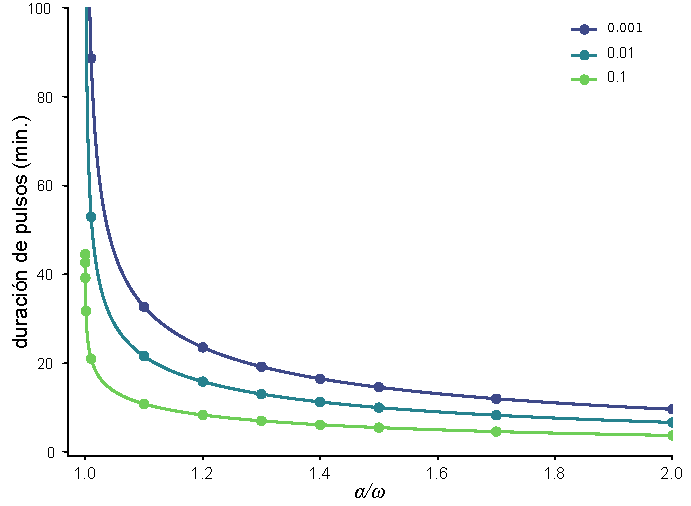
\includegraphics[width=1\columnwidth]{figures/chapter5/C5_T_exc.pdf} 
    \caption{\textbf{La duración de pulsos disminuye cuando el sistema se aleja de la bifurcación en el régimen excitable sin ruido.} Se grafica la duración de pulsos del sistema dinámico determinista \ref{C5_eq:adler_determinista} en función del cociente entre la amplitud de modulación y la frecuencia del uniforme \dddelta para los valores de $\epsilon$ indicados. La línea reporta el resultado de la expresión teórica y los puntos las mediciones numéricas (frecuencia de muestreo $0.00001\; min$). Parámetro: $\omega=2\pi/7\;\text{min}^{-1}$.}
    \label{C5_fig:T_exc_res}
\end{figure}


\section{El ruido blanco gaussiano regulariza la duración de pulsos en la bifurcación}
\sectionmark{El ruido regulariza la duración de pulsos en la bifurcación}
\label{C6_sec:duracion}


Queremos obtener una expresión analítica de la duración de pulsos de modelo de fase con bifurcación de ciclo infinito y ruido blanco gaussiano \ref{C6_eq:adler_white_noise}. Para el régimen excitable, en la sección \ref{C5_sec:T_exc} definimos un pulso cuando el sistema, luego de ser perturbado, sobrepasa el punto fijo inestable \xxi y realiza una excursión hacia el punto fijo estable siguiente \xxe, y calculamos su duración como el tiempo que tarda el sistema en llegar al entorno de \xxe habiendo partido del entorno de \xxi. Al agregar perturbaciones sistemáticas al sistema dinámico, para calcular la duración de pulsos no es necesario posicionarse en el entorno de los puntos fijos, puesto que es el ruido quien eventualmente perturbará al sistema dando lugar a una excursión o pulso. Si bien esto significa una ventaja, el carácter estocástico de este sistema dinámico añade cierta complejidad a la definición y al cálculo de la duración de pulsos. 


Podemos pensar a la duración de un pulso como el tiempo que tarda el sistema en alcanzar el punto fijo estable \xxe, dado que el comenzó en el punto fijo inestable \xxi y durante ese tiempo no volvió al punto fijo inestable \xxi. Como los valores que el ruido toma en cada instante de tiempo son aleatorios, hay distintas trayectorias posibles que cumplen con esta definición. Cada posible trayectoria puede dar lugar a pulsos con distinta duración. Por esto, la duración de pulsos así definida es una variable aleatoria, y su distribución de probabilidad asociada determina la posibilidad de obtener diferentes valores de duración de pulsos. Para nuestros objetivos, es suficiente estudiar cómo depende la duración de pulsos media de la intensidad del ruido. Para obtener una expresión analítica de la duración de pulsos media, es útil trabajar con el formalismo de tiempo de primer pasaje condicional. 


En general, el tiempo de primer pasaje medio para un sistema estocástico es el tiempo medio que tarda el sistema en alcanzar un determinado umbral por primera vez, dada su condición inicial \cite{Redner2001}.\marginpar{tiempo de\\primer pasaje\\condicional medio} De esta definición, el tiempo de primer pasaje condicional medio es el tiempo medio que tarda el sistema en alcanzar un determinado umbral de llegada por primera vez dada su condición inicial, y dado que no cruzó un umbral prohibido en el trayecto. Para nuestro problema, en el régimen excitable definimos el \textbf{tiempo de primer pasaje condicional medio} $\tplus(\xx)$ como el tiempo que le toma al sistema alcanzar el punto fijo estable \xxe por primera vez, dado que salió de \xx y nunca pasó por el punto fijo inestable \xxi. Con esta idea, definimos la \textbf{duración de pulsos media} $T_\xi$ en el excitable como el tiempo medio que tarda el sistema en llegar a al punto fijo estable \xxe, habiendo salido pero nunca vuelto a pasar por el punto fijo inestable \xxi, es decir,\marginpar{duración de\\pulsos media}
\begin{align}
    T_\xi = \lim_{\xx \rightarrow \xxi}\tplus(\xx).
    \label{C6_eq:Txi_def}
\end{align}
Elegimos en este caso anotar la duración de pulsos con el subíndice $\xi$ para reforzar que corresponde a la definición propuesta para el modelo con ruido. Para el caso oscilatorio, es intuitivo pensar que la duración de pulsos media es el tiempo medio que tarda el sistema en alcanzar $\xx_0+2\pi$, habiendo salido y no vuelto a $\xx_0$. Este problema también es un problema de tiempo de primer pasaje condicional, y es trivial extender la definición \ref{C6_eq:Txi_def} a este régimen reemplazando $\xxi \rightarrow \xx_0$ y $\xxe \rightarrow \xx_0+2\pi$, donde $\xx_0$ es cualquier valor inicial de la fase. Por simplicidad, trabajaremos con la notación \ref{C6_eq:Txi_def} más amigable para el régimen excitable, y luego haremos los reemplazos correspondientes para estudiar la duración de pulsos media en el régimen oscilatorio. 


Para obtener una expresión analítica de la duración de pulsos media, utilizaremos el formalismo de Laplace, es decir, la versión integrada de la ecuación de tiempo de primer pasaje condicional \cite{Redner2001}. Comenzaremos por obtener una expresión para el tiempo de primer pasaje condicional medio, primero obteniendo una ecuación diferencial para esta variable y luego su solución. Finalmente, tomaremos el límite \ref{C6_eq:Txi_def} para obtener la duración de pulsos.

\subsection{Ecuación diferencial para el tiempo de primer pasaje condicional medio}
\subsectionmark{Tiempo de primer pasaje condicional medio}

Comenzamos definiendo $\epsplus(\xx)$ como la probabilidad de que el sistema llegue al punto fijo estable \xxe sin pasar por el punto fijo inestable \xxi, habiendo salido de \xx contenido en $[ \,\xxi,\xxe ]\,$. Podemos calcular a $\epsplus(\xx)$ como \marginpar{probabilidad\\condicional \epsplus(\xx)}
\begin{equation}
    \epsplus(\xx) = \sum_{p_{+}} P_{p_{+}}(\xx),
    \label{C6_eq:mFPT_eps_def}
\end{equation}
donde $P_{p_{+}}(\xx)$ es la probabilidad de una única trayectoria $p_{+}$ que comienza en \xx llegue a \xxe evitando \xxi. Para encontrar una ecuación diferencial para \epsplus(\xx), comenzaremos por trabajar con un problema de \textit{random walk} unidimensional no simétrico a primeros vecinos en el intervalo finito $[\xxi,\xxe ]$, y más adelante tomaremos el límite al continuo\marginpar{problema de\\\textit{random walk}}. Un problema de \textit{random walk} es un proceso aleatorio que describe una trayectoria que consiste en una sucesión de pasos aleatorios. Entonces, imaginemos que el sistema se encuentra en \xx. Si consideramos el problema unidimensional y a primeros vecinos, el sistema puede moverse solamente un paso a la izquierda o un paso a la derecha en un instante de tiempo. Entonces, en un instante de tiempo posterior, el sistema se encontrará en $\xx+\deltax$ con una probabilidad $q(\xx)$, y en $\xx-\deltax$ con una probabilidad $1-q(\xx)$, donde la función $q(\xx)$ determina la asimetría del \textit{random walk}. Esta propiedad es fácil de ver en el límite de \textit{random walk} simétrico, donde $q(\xx) = 1/2$ y el sistema tiene la misma probabilidad de estar un paso adelante $\xx+\deltax$ y un paso atrás $\xx-\deltax$. En cambio, para otros valores de $q(\xx)$, el sistema tendrá una probabilidad distinta de estar un paso adelante que un paso atrás. Como agregado, proponemos la posibilidad de que $q(\xx)$ dependa de la localización del sistema \xx, pero que sea independiente del tiempo. Con esta interpretación, podemos reexpresar $ \epsplus(\xx)$ separando explícitamente el primer paso de todas las trayectorias,
\begin{align}
    \epsplus(\xx) &= \sum_{p_{+}} \left( q(\xx) P_{p_{+}}(\xx + \deltax) + \left(1-q(\xx)\right) P_{p_{+}}(\xx - \deltax) \right) \nonumber \\
    & = q(\xx) \epsplus(\xx+\deltax) +  \left(1-q(\xx)\right) \epsplus(\xx - \deltax) 
    \label{C6_eq:mFPT_eps_S1}.
\end{align}
Si asumimos que \deltax es pequeño comparado con \xx, podemos desarrollar en series la expresión \ref{C6_eq:mFPT_eps_S1}, y
\begin{align}
    \epsplus(\xx) = & q(\xx) \left[  \epsplus(\xx) + \epsplus'(\xx) \; \deltax + \epsplus''(\xx) \; \frac{\deltax^2}{2} \right] + \nonumber \\  & \left(1-q(\xx)\right) \left[  \epsplus(\xx) - \epsplus'(\xx) \; \deltax + \epsplus''(\xx) \; \frac{\deltax^2}{2} \right].
\end{align}
Luego,
\begin{align}
    \epsplus(\xx) &=  \epsplus(\xx) + \big(2q(\xx)-1\big) \epsplus'(\xx) \; \deltax + \epsplus''(\xx) \; \frac{\deltax^2}{2} \nonumber \\
    0 &=  (2q(\xx)-1) \epsplus'(\xx) \; \deltax + \epsplus''(\xx) \; \frac{\deltax^2}{2}. \label{C6_eq:mFPT_eps_S2}
\end{align}
La expresión \ref{C6_eq:mFPT_eps_S2} no es más que una ecuación diferencial para $\epsplus(\xx)$. Antes de tomar el límite al continuo, dividimos a la expresión \ref{C6_eq:mFPT_eps_S2} por el incremento temporal $\delta t$,
\begin{align}
     0 =  \big(2q(\xx)-1\big) \epsplus'(\xx) \; \frac{\deltax}{\delta t} + \epsplus''(\xx) \; \frac{\deltax^2}{2 \delta t}. 
     \label{C6_eq:mFPT_eps_S3}
\end{align}
Para tomar el límite al continuo, donde $\delta t \rightarrow   0 $ y $\deltax \rightarrow 0$, es útil definir
\begin{equation}
    v(\xx) = \big(2q(\xx)-1\big) \frac{\deltax}{\delta t} \qquad D = \frac{\deltax^2}{2 \delta t} \qquad \text{con} \; \delta t \rightarrow   0 \; \text{y} \; \deltax \rightarrow 0 .
    \label{C6_eq:mFPT_eps_def_vD}
\end{equation}
Si incorporamos esta definición a la expresión \ref{C6_eq:mFPT_eps_S3},
\begin{align}
     0 &=  v(\xx) \epsplus'(\xx) + D \epsplus''(\xx) .
     \label{C6_eq:mFPT_eps_S4}
\end{align}
Luego, conseguimos una ecuación diferencial que describe $\epsplus(\xx)$, en donde aún desconocemos $v(\xx)$ y $D$. Para escribir una expresión para estos coeficientes, definimos $P(\xx,t)$ como la probabilidad de estar en \xx a tiempo $t$. Siguiendo un razonamiento análogo al anterior, podemos escribir a la probabilidad de estar en \xx a tiempo $t+\delta t$ operando sobre sus contribuciones: (i) la probabilidad de haber hecho un paso hacia adelante desde $\xx-\deltax$ en el instante t, sumado a (ii) la probabilidad de haber hecho un paso hacia atrás desde $\xx+\deltax$ en el instante t, más (iii) la probabilidad de estar en \xx en el instante t y no realizar ningún movimiento, menos (iv) la probabilidad de originalmente estar en \xx a tiempo t y moverse para adelante y (v) para atrás, tal que 
\begin{align}
    P(\xx,t + \delta t ) &=  q(\xx - \deltax) P(\xx-\deltax,t) + \left(1-q(\xx + \deltax)\right) P(\xx+\deltax,t) \nonumber \\ +& P(\xx,t) - q(\xx) P(\xx,t) - \left(1-q(\xx)\right) P(\xx,t).
    \label{C6_eq:mFPT_eps_S5}
\end{align}
Otra vez, podemos asumir que \deltax es pequeño comparado con \xx y expandir a la expresión \ref{C6_eq:mFPT_eps_S5} en una serie de potencias a segundo orden, 
\begin{align}
    & P( \xx,t + \delta t) - P(\xx,t) = \nonumber \\
    & \left[ q(\xx) - q'(\xx)\deltax + q''(\xx) \frac{\deltax^2}{2}  \right] \left[ P(\xx,t) - \partial_\xx P(\xx,t) \deltax + \partial_{\xx \xx} P(\xx,t) \frac{\deltax^2}{2}  \right] \nonumber \\ & + \left[ 1 - q(\xx) - q'(\xx)\deltax - q''(\xx) \frac{\deltax^2}{2}  \right] \left[ P(\xx,t) + \partial_\xx P(\xx,t) \deltax + \partial_{\xx \xx} P(\xx,t) \frac{\deltax^2}{2}  \right] \nonumber \\ & - P(\xx,t) .
\end{align}
Luego, 
\begin{align}
    & P( \xx,t + \delta t) - P(\xx,t) = \nonumber \\
    & P(\xx,t) \left[ q(\xx) - q'(\xx)\deltax + q''(\xx) \frac{\deltax^2}{2} + 1 - q(\xx) - q'(\xx)\deltax - q''(\xx) \frac{\deltax^2}{2} -1\right] \nonumber \\ & + \partial_\xx P(\xx,t) \; \deltax \; \left[ - q(\xx) + q'(\xx)\deltax - q''(\xx) \frac{\deltax^2}{2} + 1 - q(\xx) - q'(\xx)\deltax - q''(\xx) \frac{\deltax^2}{2}\right] \nonumber \\ &+ \partial_{\xx \xx} P(\xx,t) \;  \frac{\deltax^2}{2} \; \left[  q(\xx) - q'(\xx)\deltax + q''(\xx) \frac{\deltax^2}{2} +  1 - q(\xx) - q'(\xx)\deltax - q''(\xx) \frac{\deltax^2}{2} \right] .
\end{align}
Si simplificamos la expresión que conseguimos, 
\begin{align}
     & P( \xx,t + \delta t) - P(\xx,t) = \nonumber \\
     & - 2 q'(\xx) \; \deltax \; P(\xx,t) + \left[ 1- 2 q(\xx) - q''(\xx) \deltax^2 \right] \; \deltax \; \partial_\xx P(\xx,t) \nonumber \\ & +\left[ 1-2 q'(\xx) \deltax \right] \frac{\deltax^2}{2}\partial_{\xx \xx} P(\xx,t)  .
     \label{C6_eq:mFPT_eps_S6}
\end{align}
Como estamos considerando términos hasta el segundo orden, despreciamos los proporcionales a $\deltax^3$. Si luego dividimos \ref{C6_eq:mFPT_eps_S6} por el incremento temporal $\delta t$,
\begin{align}
    & \frac{P( \xx,t + \delta t) - P(\xx,t)}{\delta t}  = \nonumber \\ & - 2 q'(\xx) \frac{\deltax}{\delta t} P(\xx,t) + \left[ 1- 2 q(\xx) \right] \frac{\deltax}{\delta t} \partial_\xx P(\xx,t) +  \frac{\deltax^2}{2 \delta t}\partial_{\xx \xx} P(\xx,t).
    \label{C6_eq:mFPT_eps_S7}
\end{align}
Teniendo en cuenta que 
\begin{align}
    \partial_\xx\left( \left(1-2q(\xx)\right) \frac{\deltax}{\delta t} \right) = - 2 q'(\xx) \frac{\deltax}{\delta t}, \nonumber
\end{align}
podemos reescribir la expresión \ref{C6_eq:mFPT_eps_S7} como 
\begin{align}
    \frac{P( \xx,t + \delta t)  - P(\xx,t) }{\delta t} &= - \partial_\xx \left[ (2q(\xx)-1) \frac{\deltax}{\delta t} P(\xx,t) \right] + \frac{\deltax^2}{2 \delta t}\partial_{\xx \xx} P(\xx,t). 
\end{align}
Finalmente, tomamos el límite al continuo y redefinimos según \ref{C6_eq:mFPT_eps_def_vD}, 
\begin{align}
   \partial_t P(\xx,t) &= - \partial_\xx \left[ v(\xx) P(\xx,t) \right] + D \partial_{\xx \xx} P(\xx,t).
   \label{C6_eq:mFPT_eps_S8}
\end{align}
La ecuación \ref{C6_eq:mFPT_eps_S8} se trata de la ecuación de Fokker Planck para un proceso homogéneo, donde el \textit{drift} $v(\xx)$ y la difusión $D$ son independientes del tiempo. El proceso estocástico que describe la solución de la ecuación \ref{C6_eq:mFPT_eps_S8} es equivalente al que describe la ecuación diferencial estocástica de Itô \cite{Gardiner}
\begin{equation}
    \partial_t  \theta(t) =  v(\xx) + \sqrt{2D} \xi_w(t).
\end{equation}
Comparando esta ecuación diferencial con \ref{C6_eq:adler_white_noise}, es fácil determinar que 
\begin{align}
    v(\xx) = \omega + \alpha \sin{(\xx)}  \label{C6_eq:mFPT_eps_def_vD_solved}
\end{align}
y $D$ es la intensidad del ruido. Una vez escrita una expresión para los coeficientes $v(\xx)$ y $D$, podemos finalmente escribir la ecuación diferencial que describe $\epsplus(\xx)$ a partir de reemplazar a estos coeficientes en \ref{C6_eq:mFPT_eps_S4}
\begin{align}
     0 &=  \left(\omega + \alpha \sin{(\xx)}\right) \epsplus'(\xx) + D \epsplus''(\xx) .
     \label{C6_eq:mFPT_eps_eq_res}
\end{align}
Recordemos que la $\epsplus(\xx)$ es la probabilidad de que el sistema llegue al punto fijo estable \xxe sin pasar por el punto fijo inestable \xxi, habiendo salido de $ \xx  \in [ \,\xxi,\xxe ]\,$. Luego, por definición, la probabilidad de que el sistema llegue al punto fijo estable \xxe sin pasar por el punto fijo inestable \xxi habiendo salido de \xxi es nula. Además, la probabilidad de que el sistema llegue al punto fijo estable \xxe sin pasar por el punto fijo inestable \xxi habiendo salido de \xxe es uno. Estos dos casos triviales constituyen las condiciones de contorno de \ref{C6_eq:mFPT_eps_eq_res}
\begin{align}
    \epsplus(\xxi) = 0 \qquad \epsplus(\xxe) = 1.
    \label{C6_eq:mFPT_eps_cdc}
\end{align}
% VER comentar sobre el análogo electrostático?


Ahora, estamos en condiciones de intentar derivar una ecuación diferencial para el tiempo de primer pasaje condicional medio $\tplus(\xx)$. Formalmente, definimos el tiempo de primer pasaje condicional medio $\tplus(\xx)$ como el tiempo medio que tarda el sistema en llegar al punto fijo estable \xxe sin haber pasado por el punto fijo inestable \xxi, habiendo salido de \xx contenido en $[ \,\xxi,\xxe ]\,$. Si pensamos que $t_{p_{+}}(\xx)$ es el tiempo que tarda una trayectoria posible $p_{+}$ en realizar el recorrido y $P_{p_{+}}$ la probabilidad de que cada una de esas posibles trayectorias ocurra,
\begin{align}
    \tplus(\xx) = \frac{\sum_{p_{+}}p_{+}(\xx) t_{p_{+}}(\xx)}{\sum_{p_{+}}p_{+}(\xx)} = \frac{\sum_{p_{+}}p_{+}(\xx) t_{p_{+}}(\xx)}{\epsplus(\xx)},
\end{align}
en donde para calcular el valor medio dividimos sobre la suma de probabilidades de las trayectorias posibles, y luego usamos la definición \ref{C6_eq:mFPT_eps_def}. Luego,
\begin{align}
    \tplus(\xx) \epsplus(\xx)  &= \sum_{p_{+}}p_{+}(\xx) t_{p_{+}}(\xx).
    \label{C6_eq:mFPT_tplus_def}
\end{align}
Con un razonamiento análogo al realizado para obtener la ecuación \ref{C6_eq:mFPT_eps_S1}, podemos reexpresar $\tplus(\xx) \epsplus(\xx)$ separando explícitamente el primer paso de todas las trayectorias,  
\begin{align}
   & \tplus(\xx) \epsplus(\xx) = \sum_{p_{+}} \Big[ q(\xx)  p_{+}(\xx + \deltax ) \left( t_{p_{+}}(\xx + \deltax) + \delta t \right)  \nonumber \\ & + \big( 1 - q(\xx) \big)  p_{+}(\xx - \deltax ) \left( t_{p_{+}}(\xx - \deltax) + \delta t \right)\Big] \nonumber \\
   & =  q(\xx) \sum_{p_{+}} p_{+}(\xx + \deltax ) t_{p_{+}}(\xx + \deltax) + q(\xx) \sum_{p_{+}} p_{+}(\xx + \deltax ) \delta t  \nonumber \\ & + \big( 1 - q(\xx) \big) \sum_{p_{+}}p_{+}(\xx - \deltax ) t_{p_{+}}(\xx - \deltax) +  \big( 1 - q(\xx) \big) \sum_{p_{+}}p_{+}(\xx - \deltax ) \delta t .
\end{align}
Usamos las definiciones \ref{C6_eq:mFPT_tplus_def} y \ref{C6_eq:mFPT_eps_def} para reemplazar las sumatorias
\begin{align}
   \tplus(\xx) \epsplus(\xx) & = q(\xx) \tplus(\xx + \deltax) \epsplus(\xx + \deltax) + q(\xx) \epsplus(\xx + \deltax) \delta t \nonumber \\ & + \big( 1 - q(\xx) \big) \tplus(\xx - \deltax) \epsplus(\xx - \deltax) +  \big( 1 - q(\xx) \big) \epsplus(\xx - \deltax) \delta t.
   \label{C6_eq:mFPT_tplus_S1}
\end{align}
Para simplificar la lectura, definimos  $\epstplus(\xx) =  \tplus(\xx) \epsplus(\xx)$, y \ref{C6_eq:mFPT_tplus_S1} queda escrita como
\begin{align}
   \epstplus(\xx) & = q(\xx) \epstplus(\xx + \deltax) + q(\xx) \epsplus(\xx + \deltax) \delta t \nonumber \\ & + \big( 1 - q(\xx) \big) \epstplus(\xx - \deltax) +  \big( 1 - q(\xx) \big) \epsplus(\xx - \deltax) \delta t.
   \label{C6_eq:mFPT_tplus_S2}
\end{align}
Si nuevamente consideramos $\deltax \ll \xx$, podemos realizar el desarrollo en series de \ref{C6_eq:mFPT_tplus_S2} hasta segundo orden en \deltax. Para construir este desarrollo en series, comenzamos por expresar los primeros órdenes de $\epstplus(\xx)$ y $\epsplus(\xx)$ 
\begin{align}
    \epstplus(\xx \pm \deltax) & = \epstplus(\xx) \pm \epstplus'(\xx) \deltax + \epstplus''(\xx) \frac{\deltax^2}{2} \nonumber \\
    \epsplus(\xx \pm \deltax) & = \epsplus(\xx) \pm \epsplus'(\xx) \deltax + \epsplus''(\xx) \frac{\deltax^2}{2}.
\end{align}
Si reemplazamos estas cantidades en \ref{C6_eq:mFPT_tplus_S2},
\begin{align}
       & \epstplus(\xx) = q(\xx) \Bigg[  \epstplus(\xx) + \epstplus'(\xx) \deltax + \epstplus''(\xx) \frac{\deltax^2}{2} \Bigg] + q(\xx) \delta t \Bigg[  \epsplus(\xx) + \epsplus'(\xx) \deltax + \epsplus''(\xx) \frac{\deltax^2}{2}\Bigg] \nonumber \\ & +  \big( 1 - q(\xx) \big) \Bigg[  \epstplus(\xx) - \epstplus'(\xx) \deltax + \epstplus''(\xx) \frac{\deltax^2}{2} \Bigg] \nonumber \\ & + \big( 1 - q(\xx) \big) \delta t \Bigg[  \epsplus(\xx) - \epsplus'(\xx) \deltax + \epsplus''(\xx) \frac{\deltax^2}{2}\Bigg] .
\end{align}
Simplificando,
\begin{align}
        \epstplus(\xx) & = \epstplus(\xx) + \big(2 q(\xx) -1 \big) \; \deltax \;  \epstplus'(\xx)  +  \frac{\deltax^2}{2}  \epstplus''(\xx) \nonumber \\ & + \delta t \; \epsplus(\xx)  - \big(2 q(\xx) -1 \big) \; \deltax \; \delta t \;  \epsplus'(\xx) +  \frac{\deltax^2}{2} \; \delta t \; \epsplus''(\xx) .
        \label{C6_eq:mFPT_tplus_S3}
\end{align}
Si dividimos toda la expresión \ref{C6_eq:mFPT_tplus_S3} por el incremento temporal $\delta t$, y luego tomamos el límite al continuo  $\delta t \rightarrow   0 $ y $\deltax \rightarrow 0$, 
\begin{align}
       0 &= v(\xx) \epstplus'(\xx)  + D \epstplus''(\xx) + \epsplus(\xx) \nonumber\\
       -\epsplus(\xx) &= v(\xx) \epstplus'(\xx)  + D \epstplus''(\xx),
\end{align}
en donde utilizamos el resultado \ref{C6_eq:mFPT_eps_S4} y las definiciones de \ref{C6_eq:mFPT_eps_def_vD}.
Finalmente, logramos obtener una ecuación diferencial para el producto $\epstplus(\xx) = \epsplus(\xx) \tplus(\xx)$, y
\begin{align}
       - \epsplus(\xx) &= v(\xx) \big(\epsplus(\xx) \tplus(\xx)\big)'  + D  \big(\epsplus(\xx) \tplus(\xx)\big)''  \nonumber \\
     - \epsplus(\xx) &= \big(\omega + \alpha \sin{(\xx)}\big) \big(\epsplus(\xx) \tplus(\xx)\big)'  + D \big(\epsplus(\xx) \tplus(\xx)\big)'' ,
       \label{C6_eq:mFPT_tplus_eq_res}
\end{align}
donde en la última ecuación utilizamos la expresión  \ref{C6_eq:mFPT_eps_def_vD_solved}.

De \ref{C6_eq:mFPT_eps_cdc} sabemos que $\epsplus(\xx)$ se anula en \xxi, por ende el producto $\epsplus(\xx) \tplus(\xx)$ también lo hará. Por otro lado, recordemos que $\tplus(\xx)$ era el tiempo medio que tarda el sistema en llegar al punto fijo estable \xxe sin haber pasado por el punto fijo inestable \xxi, habiendo salido de \xx. Luego, es trivial que $\tplus(\xx)$ se anula en \xxe. Con estas dos características, tenemos las condiciones de contorno correspondientes a la ecuación diferencial \ref{C6_eq:mFPT_tplus_eq_res}
\begin{align}
    \epsplus(\xxe) \tplus(\xxe) = 0 \qquad \epsplus(\xxi) \tplus(\xxi) = 0 .
    \label{C6_eq:mFPT_tplus_eq_cdc}
\end{align}

Resolviendo las ecuaciones \ref{C6_eq:mFPT_tplus_eq_res} y \ref{C6_eq:mFPT_tplus_eq_cdc}, junto con \ref{C6_eq:mFPT_eps_eq_res} y \ref{C6_eq:mFPT_eps_cdc} podremos encontrar una expresión analítica para el tiempo de primer pasaje condicional medio \tplus(\xx). 

%no entiendo si poner o no el tema de el FPT no condicional

\subsection{Expresión analítica del tiempo de primer pasaje condicional medio}

Como primer paso, buscaremos obtener una expresión analítica para la probabilidad condicional $\epsplus(\xx)$. Porque la notación es más sencilla, resolveremos la ecuación \ref{C6_eq:mFPT_eps_S4} con condiciones de contorno \ref{C6_eq:mFPT_eps_cdc}, y luego haremos el reemplazo \ref{C6_eq:mFPT_eps_def_vD_solved} correspondiente para encontrar la solución de la ecuación \ref{C6_eq:mFPT_eps_eq_res}. De \ref{C6_eq:mFPT_eps_S4},
\begin{align}
     \frac{\epsplus''(\xx)}{\epsplus'(\xx)} = - \frac{v(\xx)}{D}.
\end{align}
Si definimos 
\begin{align*}
     f(\xx) = \epsplus'(\xx) \quad \Rightarrow \quad \frac{d f}{d\xx}(\xx) = \epsplus''(\xx),
\end{align*}
luego
\begin{align}
     \frac{df}{f(\xx)} = - \frac{v(\xx)}{D} d\xx.
     \label{C6_eq:mFPT_eps_R1}
\end{align}
Integramos a ambos lados de la ecuación \ref{C6_eq:mFPT_eps_R1}, 
\begin{align}
     \ln{(f(\xx))} = - \frac{V(\xx)}{D} + C,
\end{align}
donde $V(\xx)$ es la primitiva de $v(\xx)$, y en $C$ absorbimos todas las constantes de integración. Luego,
\begin{align}
     f(\xx) &= \frac{1}{N} e^{- \frac{V(\xx)}{D}} \nonumber \\
     \epsplus'(\xx) & =\frac{1}{N} e^{- \frac{V(\xx)}{D}}, 
     \label{C6_eq:mFPT_eps_R2}
\end{align}
donde $N$ es una constante positiva. Logramos obtener la solución homogénea de $\epsplus'(\xx)$. Para obtener una expresión para \epsplus(\xx), hay que integrar \ref{C6_eq:mFPT_eps_R2}. Elegimos los límites de integración de manera de cumplir la condición de contorno $\epsplus(\xxi) = 0 $ de \ref{C6_eq:mFPT_eps_cdc} y
\begin{align}
     \epsplus(\xx) & = \frac{1}{N} \int_{\xxi}^\xx d\xx'\; e^{- \frac{V(\xx')}{D}}  .  \label{C6_eq:mFPT_N_epsplus}
\end{align}
Para determinar $N$ utilizaremos la otra condición de contorno de \ref{C6_eq:mFPT_eps_cdc}
\begin{align}
     \epsplus(\xxe) & = \frac{1}{N} \int_{\xxi}^{\xxe} d\xx'\; e^{- \frac{V(\xx')}{D}} = 1. 
\end{align}
Luego,
\begin{align}
      N &= \int_{\xxi}^{\xxe} d\xx'\; e^{- \frac{V(\xx')}{D}} .
\end{align}
Con este resultado, logramos obtener una expresión para la probabilidad condicional $\epsplus(\xx)$ 
\begin{align}
     \epsplus(\xx) & = \frac{\int_{\xxi}^\xx d\xx'\; e^{- \frac{V(\xx')}{D}}}{\int_{\xxi}^{\xxe} d\xx'\; e^{- \frac{V(\xx')}{D}}} \nonumber \\
     \epsplus(\xx) & = \frac{\int_{\xxi}^\xx d\xx'\; e^{- \frac{\omega \xx' - \alpha \cos{(\xx')}}{D}}}{\int_{\xxi}^{\xxe} d\xx'\; e^{- \frac{\omega \xx' - \alpha \cos{(\xx')}}{D}}},
     \label{C6_eq:mFPT_eps_res}
\end{align}
en donde reemplazamos $V(\xx) = \omega \xx - \alpha \cos{(\xx)}$. Este resultado se trata de una expresión integral cuyo resultado analítico es difícil de obtener, y optamos por resolverla numéricamente.


Para analizar el resultado \ref{C6_eq:mFPT_eps_res}, es útil tomar el límite del oscilador uniforme con ruido blanco gaussiano aditivo, donde $\alpha = 0$. En el caso sin ruido, el oscilador uniforme consiste en oscilaciones de frecuencia (o velocidad de la fase) constante $\omega$, y no hay puntos fijos. Entonces, sin pérdida de generalidad podemos considerar en este caso donde hay ruido
\begin{align}
    v(\xx) = \omega \qquad 
    \xxi = 0 \qquad \xxe = 2 \pi.
    \label{C6_eq:mFPT_uniforme}
\end{align}
Con estos valores, la probabilidad $\epsplus(\xx)$ es
\begin{align}
     \epsplus(\xx) & = \frac{\int_{0}^\xx d\xx'\; e^{- \frac{\omega \xx'}{D}}}{\int_{0}^{2\pi} d\xx'\; e^{- \frac{\omega \xx'}{D}}}
      = \frac{\frac{-D}{\omega} \left[e^{- \frac{\omega \xx}{D}} - 1\right]}{\frac{-D}{\omega} \left[e^{- \frac{\omega 2\pi}{D}} - 1\right]} = \frac{ 1 - e^{- \frac{\omega \xx}{D}}}{1- e^{- \frac{\omega 2\pi}{D}}}.
\end{align}
Este límite coincide con la probabilidad condicional calculada para el oscilador armónico reportada previamente \cite{Redner2001}. Este resultado es creciente en \xx, lo que indica que cuanto más cerca de $\xxe = 2\pi$, mayor probabilidad de llegar hasta él sin cruzar antes $\xxi = 0$ . Este resultado es intuitivo, cuanto más cerca del límite \xxe del intervalo, el sistema necesita recorrer menos distancia para alcanzarlo, lo que conduce a una mayor probabilidad de éxito. Además, a mayor frecuencia del uniforme y a menor intensidad del ruido, ese crecimiento es más abrupto. Es decir, cuanto más domine la dinámica determinista por sobre el ruido, mayor probabilidad de éxito para recorrer la misma trayectoria. 

En la figura \ref{C6_fig:mFPT_eps} graficamos $\epsplus(\xx)$ en función de la condición inicial \xx. Para todos los casos, la expresión \ref{C6_eq:mFPT_eps_res} que obtuvimos está de acuerdo con las simulaciones numéricas, donde contamos cuántas trayectorias llegaban satisfactoriamente a \xxe para el sistema cuya dinámica estaba gobernada por la ecuación \ref{C6_eq:adler_white_noise} e inicialmente se encontraba en \xx. Descartamos todas las mediciones realizadas sobre las trayectorias que atravesaban \xxi y normalizamos las cuentas por el número total de simulaciones realizadas (ver apéndice \ref{C6_ap:traces}). En la figura \ref{C6_fig:mFPT_eps}A observamos que, para valores pequeños de ruido, la función $\epsplus(\xx)$ comienza siendo cercana a cero cerca del punto fijo inestable y se acerca a uno abruptamente a medida que crece la condición inicial. Este crecimiento abrupto nos informa que, para valores chicos de ruido, siempre que el sistema empiece en un entorno del punto fijo inestable, inevitablemente termina en el punto fijo estable y no vuelve al punto fijo estable, dominando la dinámica determinista por sobre la estocástica. A medida que aumenta la intensidad del ruido, $\epsplus(\xx)$ se va suavizando y pareciéndose cada vez más a la recta de pendiente unidad. Esta recta es característica de problemas de \textit{random walk} simétricos, lo que sugiere que en ese régimen la dinámica está gobernada por el ruido. En la figura \ref{C6_fig:mFPT_eps}B observamos que la probabilidad condicional $\epsplus(\xx)$ en el caso régimen oscilatorio uniforme, en el oscilatorio no-uniforme y en el excitable con valores de intensidad del ruido y frecuencia del uniforme fijos tiene la misma forma, aunque el cociente adimensional \dddelta regula localización de los puntos fijos en el régimen excitable (ecuación \ref{C5_eq:PF_def}). En la figura  \ref{C6_fig:mFPT_eps}C podemos ver que la concavidad de la probabilidad condicional $\epsplus(\xx)$ es levemente más abrupta conforme aumenta la frecuencia del uniforme $\omega$. Posiblemente esto se deba a que, cuando aumenta la frecuencia del uniforme con \dddelta y $D$ fijos, aumenta la velocidad que el sistema puede tomar dentro del intervalo $[\xxi,\xxe]$. Luego, el ruido tiene menos tiempo (o probabilidad) para perturbar al sistema hacia el punto fijo inestable. 


\begin{figure}
    \centering
    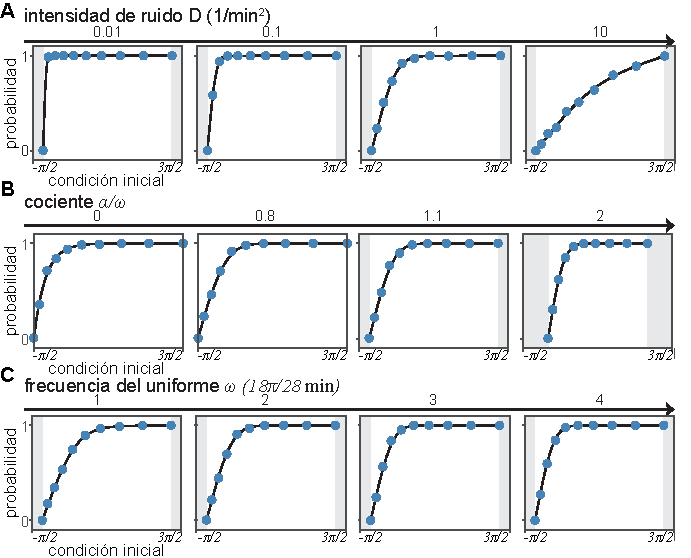
\includegraphics[width=1\columnwidth]{figures/chapter6/C6_eps_plus.pdf} 
    \caption{\textbf{Probabilidad condicional de llegar al punto fijo estable sin pasar por el inestable en función de la condición inicial.} (A) Probabilidad condicional $\epsplus(\xx)$ en función de su condición inicial \xx para distintos valores de (A) intensidad de ruido, (B) cociente adimensional \dddelta y (C) frecuencia del uniforme, indicados arriba. A menos que se especifique otro valor, $\omega = 18\pi/28 \; \text{min}^{-1}$, $\dddelta = 1.1$ y $D=1 \text{min}^{-2}$. Los puntos azules indican los resultados de los cálculos numéricos, la línea negra es el resultado de la expresión analítica \ref{C6_eq:mFPT_eps_res}, y los bordes de la región gris indican el punto fijo inestable (izquierda) o estable (derecha) si corresponde. Las simulaciones numéricas fueron $N=500$, con un paso $dt = 10^{-5}$ y una frecuencia de adquisición de $d=1$ (apéndice \ref{C6_ap:traces}).}
    \label{C6_fig:mFPT_eps}
\end{figure}


Una vez que obtuvimos la solución a \ref{C6_eq:mFPT_eps_S4}, buscamos resolver la ecuación \ref{C6_eq:mFPT_tplus_eq_res} para obtener la expresión analítica del tiempo de primer pasaje condicional medio $\tplus(\xx)$. Como \ref{C6_eq:mFPT_tplus_eq_res} es una ecuación diferencial para la derivada del producto $ \epstplus(\xx) = \epsplus(\xx) \tplus(\xx) $,  primero obtendremos una expresión para la derivada de este producto, luego integraremos la solución e impondremos las condiciones de contorno \ref{C6_eq:mFPT_tplus_eq_cdc}, para finalmente obtener la expresión analítica de  $\tplus(\xx)$. Utilizaremos el método de variación constante para dar con una expresión de \Depstplus(\xx). Como primer paso, queremos determinar la solución homogénea $\DepstplusH(\xx)$ de \ref{C6_eq:mFPT_tplus_eq_res}, y
\begin{align}
    0 &= v(\xx) \DepstplusH(\xx)  + D \DDepstplusH(\xx) \nonumber \\
    \frac{\DDepstplusH(\xx)}{\DepstplusH(\xx)} &= - \frac{v(\xx)}{D} \nonumber \\
    \DepstplusH(\xx) & = K  e^{- \frac{V(\xx)}{D}},
\end{align}
donde $V(\xx)$ es la primitiva de $v(\xx)$ y $K$ es una constante positiva.
Luego, permitimos $K \rightarrow   K(\xx)$ tal que $\Depstplus(\xx) = K(\xx) e^{- \frac{V(\xx)}{D}}$, y buscamos hallar la solución particular de \ref{C6_eq:mFPT_tplus_eq_res}
\begin{align}
    - \epsplus(\xx) &= v(\xx) \Depstplus(\xx) + D \DDepstplus(\xx) \nonumber \\
    - \epsplus(\xx) &= v(\xx) K(\xx) e^{- \frac{V(\xx)}{D}}  \nonumber \\
    & + D K'(\xx)e^{- \frac{V(\xx)}{D}} - D K(\xx) \frac{v(\xx)}{D} e^{- \frac{V(\xx)}{D}} \nonumber \\
    - \epsplus(\xx) &=  D K'(\xx)e^{- \frac{V(\xx)}{D}} .
\end{align}
Entonces
\begin{align}
         K'(\xx) = - \frac{\epsplus(\xx)}{D} e^{ \frac{V(\xx)}{D}} .
\end{align}
Para encontrar $K(\xx)$ tomamos un límite de integración arbitrario $\xx_{0}$
\begin{align}
         K(\xx) - K_0 = - \frac{1}{D} \int_{\xx_0}^\xx d\xx' \epsplus(\xx') e^{ \frac{V(\xx')}{D}},
\end{align}
donde definimos $K_0 \equiv K(\xx_0)$. Con este resultado, 
\begin{align}
    \Depstplus(\xx) = - \frac{e^{- \frac{V(\xx)}{D}}}{D} \int_{\xx_0}^\xx d\xx' \epsplus(\xx') e^{ \frac{V(\xx')}{D}} + K_0 \; e^{- \frac{V(\xx)}{D}} .
\end{align}
Luego, 
\begin{align}
   \epstplus(\xx) = - \int_{\xx_1}^{\xx} d\xx'  \frac{ e^{- \frac{V(\xx')}{D}} }{D} \int_{\xx_0}^{\xx'} d \xx'' \epsplus(\xx'') e^{ \frac{V(\xx'')}{D}} + K_0 \int_{\xx_1}^{\xx} d\xx'  e^{- \frac{V(\xx')}{D}}  .
\end{align}


Si elegimos $\xx_1 = \xxi$, utilizamos la siguiente expresión de la integral \ref{C6_eq:mFPT_N_epsplus}
\begin{align*}
    \int_{\xx_1 = \xxi}^{\xx} d\xx'  e^{- \frac{V(\xx')}{D}} = N \epsplus(\xx),
\end{align*}
y además se cumple una de las condiciones de contorno \ref{C6_eq:mFPT_tplus_eq_cdc} donde $\epstplus(\xxi) = 0$,
\begin{align}
   \epstplus(\xx) = - \int_{\xx_1}^{\xx} d\xx'  \frac{ e^{- \frac{V(\xx')}{D}} }{D} \int_{\xx_0}^{\xx'} d \xx'' \epsplus(\xx'') e^{ \frac{V(\xx'')}{D}} + N \epsplus(\xx) K_0 .
\end{align}
Si definimos 
\begin{align*}
I_0(\xx) =  -\frac{1}{D} \int_{\xx_0}^\xx d \xx' \epsplus(\xx') e^{ \frac{V(\xx')}{D}}, 
\end{align*}
es posible reescribir
\begin{align}
   \epstplus(\xx) &= \int_{\xxi}^{\xx} d\xx'  e^{- \frac{V(\xx')}{D}}  I_0(\xx')+  N \; \epsplus(\xx) \; K_0 .
   \label{C6_eq:mFPT_tplus_R1}
\end{align}
Notando que
\begin{align*}
    e^{- \frac{V(\xx)}{D}} = N \epsplus(\xx)',
\end{align*}
podemos reescribir la expresión \ref{C6_eq:mFPT_tplus_R1} usando partes para descomponer el término de la integral,
\begin{align}
   \epstplus(\xx) &= I_0(\xx') N \epsplus(\xx') \Bigg|_{\xxi}^{\xx} - \int_{\xxi}^{\xx} d\xx' N \epsplus(\xx') \Big(-\frac{1}{D} \epsplus(\xx') e^{ \frac{V(\xx')}{D}} \Big) +  N \epsplus(\xx) K_0 \nonumber \\
            &= I_0(\xx) N \epsplus(\xx) - I_0(\xxi) N \epsplus(\xxi) + \frac{N}{D} \int_{\xxi}^{\xx} d\xx'  \epsplus^2(\xx') e^{ \frac{V(\xx')}{D}} +  N \epsplus(\xx) K_0 \nonumber \\
            &= I_0(\xx) N \epsplus(\xx) + \frac{N}{D} \int_{\xxi}^{\xx} d\xx'  \epsplus^2(\xx') e^{ \frac{V(\xx')}{D}} +  N \epsplus(\xx) K_0 ,
\end{align}
donde en la última igualdad usamos $\epsplus(\xxi) = 0$. Finalmente, 
\begin{align}
   \epstplus(\xx) &= \big(I_0(\xx)+K_0\big) N \epsplus(\xx) + \frac{N}{D} \int_{\xxi}^{\xx} d\xx'  \epsplus^2(\xx') e^{ \frac{V(\xx')}{D}}.  \label{C6_eq:mFPT_aux}
\end{align}
Ahora podemos determinar las constantes $K_0$ y $\theta_0$ con las condiciones de contorno.
\begin{align}
   \epstplus(\xxe) &= \big(I_0(\xxe)+K_0\big) N \epsplus(\xxe) + \frac{N}{D} \int_{\xxi}^{\xxe} d\xx'  \epsplus^2(\xx') e^{ \frac{V(\xx')}{D}} = 0 \nonumber \\
   0&=\big(I_0(\xxe)+K_0\big) + \frac{1}{D} \int_{\xxi}^{\xxe} d\xx'  \epsplus^2(\xx') e^{ \frac{V(\xx')}{D}} \nonumber \\
   0&=-\frac{1}{D} \int_{\xx_0}^{\xxe} d \xx' \epsplus(\xx') e^{ \frac{V(\xx')}{D}} +K_0 + \frac{1}{D} \int_{\xxi}^{\xxe} d\xx'  \epsplus^2(\xx') e^{ \frac{V(\xx')}{D}} \nonumber \\
   K_0 &= \frac{1}{D} \Big( \int_{\xx_0}^{\xxe} d \xx' \epsplus(\xx') e^{ \frac{V(\xx')}{D}} - \int_{\xxi}^{\xxe} d\xx'  \epsplus^2(\xx') e^{ \frac{V(\xx')}{D}}\Big)
\end{align}
Si elegimos $\xx_0 = \xxe$,
\begin{align}
   K_0 &= -\frac{1}{D} \int_{\xxi}^{\xxe} d\xx'  \epsplus^2(\xx') e^{ \frac{V(\xx')}{D}}.
\end{align}
Para terminar, podemos reemplazar a $K_0$ e $I_0$ en la ecuación \ref{C6_eq:mFPT_aux} por sus expresiones, y
\begin{align}
   \epstplus(\xx) &= - \frac{N}{D} \epsplus(\xx) \Big(  \int_{\xx_e}^\xx d \xx' \epsplus(\xx') e^{ \frac{V(\xx')}{D}} +  \int_{\xxi}^{\xxe} d\xx'  \epsplus^2(\xx') e^{ \frac{V(\xx')}{D}} \nonumber \\ & - \frac{1}{\epsplus(\xx)} \int_{\xxi}^{\xx} d\xx'  \epsplus^2(\xx') e^{ \frac{V(\xx')}{D}} \Big) \nonumber \\
     \epstplus(\xx) &= \frac{N}{D} \epsplus(\xx) \Big(  \int_\xx^{\xx_e} d \xx' \epsplus(\xx') e^{ \frac{V(\xx')}{D}} -  \int_{\xxi}^{\xxe} d\xx'  \epsplus^2(\xx') e^{ \frac{V(\xx')}{D}} \nonumber \\ & + \frac{1}{\epsplus(\xx)} \int_{\xxi}^{\xx} d\xx'  \epsplus^2(\xx') e^{ \frac{V(\xx')}{D}} \Big).
\end{align}
Finalmente, logramos obtener la expresión analítica para el tiempo de primer pasaje condicional medio
\begin{align}
     \tplus(\xx)&= \frac{N}{D} \Big(  \int_\xx^{\xx_e} d \xx' \epsplus(\xx') e^{ \frac{V(\xx')}{D}} -  \int_{\xxi}^{\xxe} d\xx'  \epsplus^2(\xx') e^{ \frac{V(\xx')}{D}} + \frac{1}{\epsplus(\xx)} \int_{\xxi}^{\xx} d\xx'  \epsplus^2(\xx') e^{ \frac{V(\xx')}{D}} \Big). \label{C6_eq:mFPT_tplus_res}
\end{align}
Este resultado se trata de una expresión integral cuyo resultado analítico es difícil de obtener, y optamos por resolverla numéricamente.


En el límite del oscilador uniforme \ref{C6_eq:mFPT_uniforme}, el tiempo de primer pasaje condicional medio es 
\begin{align}
     \tplus(\xx)& = \frac{2 \pi \left(e^{\frac{2 \pi \omega}{D}}+1\right) \left(e^{\frac{\omega \xx}{D}}-1\right)-\xx\left(e^{\frac{2 \pi\omega}{D}}-1\right) \left(e^{\frac{\omega \xx}{D}}+1\right)}{\omega \left(e^{\frac{2 \pi \omega}{D}}-1\right) \left(e^{\frac{\omega \xx}{D}}-1\right)},
     \label{C6_eq:mFPT_tplus_res_alpha_cero} 
\end{align}
expresión que coincide con resultados previamente reportados para el tiempo de primer pasaje condicional medio para el oscilador uniforme \cite{Redner2001}. De esta expresión, observamos que cuando la intensidad de ruido tiende a cero, \ref{C6_eq:mFPT_tplus_res_alpha_cero} tiende a $(2\pi - \xx)/\omega$, y cuando la condición inicial es $0$, el tiempo coincide con el período del oscilador uniforme. Luego, el segundo término de \ref{C6_eq:mFPT_tplus_res_alpha_cero} es la corrección correspondiente a empezar en cualquier lugar \xx del círculo. 

En la figura \ref{C6_fig:mFPT_tplus} observamos que nuestra expresión \ref{C6_eq:mFPT_tplus_res} coincide con los resultados obtenidos en simulaciones numéricas, donde medimos cuánto tiempo tardaba el sistema cuya dinámica estaba gobernada por la ecuación \ref{C6_eq:adler_white_noise} e inicialmente se encontraba en \xx en llegar a \xxe. En estas mediciones descartamos todas las mediciones que fueron realizadas sobre las trayectorias que atravesaban \xxi (ver apéndice \ref{C6_ap:traces}). Además, observamos en la figura \ref{C6_fig:mFPT_tplus} que en todos los casos el tiempo de primer pasaje medio condicional decrece conforme aumenta la condición inicial. Por otro lado, a diferencia del caso sin ruido donde si considerábamos el punto fijo inestable como la condición inicial el tiempo divergía (sección de la sección \ref{C5_sec:T_exc}), en este caso es finito y depende de los parámetros del modelo. Este comportamiento nos indica que el límite \ref{C6_eq:Txi_def} que define la duración de pulsos media del sistema \ref{C6_eq:adler_white_noise} es finito. En \ref{C6_fig:mFPT_tplus}A podemos observar que el ruido tiende a disminuir el tiempo de primer pasaje condicional medio. En las figuras \ref{C6_fig:mFPT_tplus}B y C observamos que el cociente adimensional \dddelta y la frecuencia del uniforme tienen el mismo efecto, pues la velocidad que el sistema puede tener en el intervalo $[\xxi,\xxe]$ aumenta con el cociente \dddelta y con $\omega$, y en el caso de variar \dddelta también la distancia entre la condición inicial \xx y el punto fijo estable disminuye. 



\begin{figure}
    \centering
    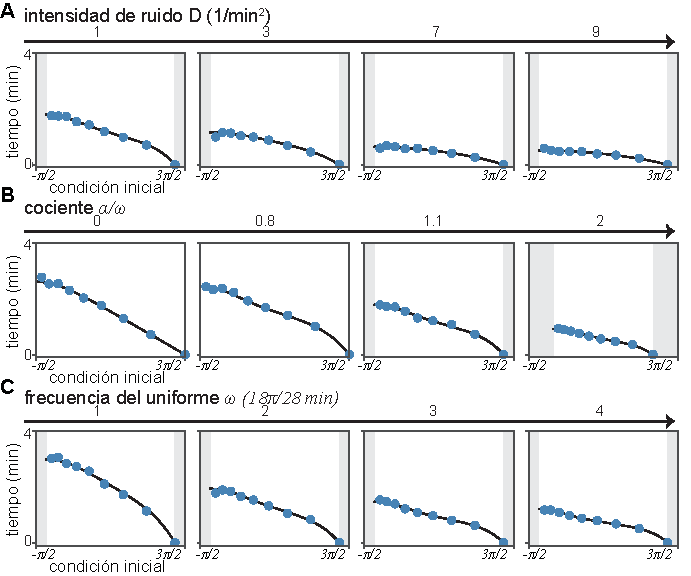
\includegraphics[width=1\columnwidth]{figures/chapter6/C6_t_plus.pdf} 
    \caption{\textbf{Tiempo medio para llegar al punto fijo estable sin pasar por el punto fijo inestable en función de la condición inicial.} (A) Tiempo medio $\tplus(\xx)$ en función de su condición inicial \xx para distintos valores de (A) intensidad de ruido, (B) cociente adimensional \dddelta y (C) frecuencia del uniforme, indicados arriba. A menos que se especifique otro valor, $\omega = 18\pi/28 \; \text{min}^{-1}$, $\dddelta = 1.1$ y $D=1 \text{min}^{-2}$. Los puntos azules indican los resultados de los cálculos numéricos, la línea negra indica el resultado de la expresión analítica \ref{C6_eq:mFPT_tplus_res}, y los bordes de la región gris indican el punto fijo inestable (izquierda) o estable (derecha) si corresponde. Las simulaciones numéricas fueron $N=500$, con un paso $dt = 10^{-5}$ y una frecuencia de adquisición de $d=1$ (apéndice \ref{C6_ap:traces}).}
    \label{C6_fig:mFPT_tplus}
\end{figure}

\subsection{Expresión analítica para la duración de pulsos media}
\sectionmark{Duración de pulsos media}

En la sección anterior observamos que el límite \ref{C6_eq:Txi_def} que define la duración de pulsos media del sistema \ref{C6_eq:adler_white_noise} es finito y depende de los parámetros del modelo. Para estudiar en detalle esta dependencia, en esta sección queremos obtener una expresión analítica para la duración de pulsos media $T_\xi$, que definimos como el tiempo medio que tarda el sistema en llegar a \xxe, habiendo salido pero nunca vuelto a pasar por \xxi.


Comenzamos por reescribir la ecuación \ref{C6_eq:mFPT_tplus_res} para tener una expresión con límites de integración más sencillos,
\begin{align}
     \tplus(\xx)&= \frac{N}{D} \Bigg(  \int_\xx^{\xx_e} d \xx' \epsplus(\xx') e^{ \frac{V(\xx')}{D}} -  \int_{\xxi}^{\xxe} d\xx'  \epsplus^2(\xx') e^{ \frac{V(\xx')}{D}} \nonumber \\ & + \frac{1}{\epsplus(\xx)} \int_{\xxi}^{\xx} d\xx'  \epsplus^2(\xx') e^{ \frac{V(\xx')}{D}} \Bigg) \nonumber \\
     &= \frac{N}{D} \Bigg[  \int_\xx^{\xx_e} d \xx' \epsplus(\xx') e^{ \frac{V(\xx')}{D}} \big(1 - \epsplus(\xx') \big)+ \nonumber \\ & \Big( \frac{1}{\epsplus(\xx)} -1 \Big) \int_{\xxi}^{\xx} d\xx'  \epsplus^2(\xx') e^{ \frac{V(\xx')}{D}} \Bigg]. \label{C6_eq:Txi_tplus_terminos}
\end{align}
Tenemos una expresión que es la suma de dos integrales. Comenzaremos por trabajar con el primer término 
\begin{align}
     \lim_{\xx \rightarrow   \xxi }&\frac{N}{D}  \int_\xx^{\xxe} d \xx' \epsplus(\xx') e^{ \frac{V(\xx')}{D}} \big(1 - \epsplus(\xx') \big) \nonumber \\
     &= \frac{N}{D} \int_{\xxi}^{\xxe} d \xx' \epsplus(\xx') e^{ \frac{V(\xx')}{D}} \big(1 - \epsplus(\xx') \big),
     \label{C6_eq:Txi_LI1}
\end{align}
donde el límite es finito. Luego, detengámonos en el segundo término de \ref{C6_eq:Txi_tplus_terminos}. Es fácil ver que la integral de este término tiende a cero cuando $\xx \rightarrow \xxi $, pues el límite de integración superior tiende al límite de integración inferior y su argumento es finito en el intervalo de integración. Esto mismo ocurre con $\epsplus(\xx)$. Según su expresión analítica \ref{C6_eq:mFPT_eps_res}, $\epsplus(\xx) \rightarrow 0$ cuando $\xx \rightarrow \xxi $. Luego, el cociente entre la integral y $\epsplus(\xx)$ da lugar a la indeterminación 
\begin{align}
      \lim_{\xx \rightarrow   \xxi }& \frac{1}{\epsplus(\xx)}  \int_{\xxi}^{\xx} d\xx'  \epsplus^2(\xx') e^{ \frac{V(\xx')}{D}}.
     \label{C6_eq:Txi_LI2_S1}
\end{align}
A partir de \ref{C6_eq:mFPT_eps_res}, podemos determinar que 
\begin{align}
     \epsplus'(\xx) & = \frac{e^{- \frac{V(\xx)}{D}}}{N},
\end{align}
y en particular 
\begin{align}
     \epsplus'(\xxi) & = \frac{e^{- \frac{V(\xxi)}{D}}}{N} = \frac{e^{- \frac{\omega \xxi - \alpha \cos{(\xxi)}}{D}}}{N} \neq 0. \nonumber 
\end{align}
Luego, como $\epsplus'(\xxi)$ no se anula ni en \xxi ni en su entorno, podemos usar la regla de L'Hospital para salvar la indeterminación \ref{C6_eq:Txi_LI2_S1}
\begin{align}
     & \lim_{\xx \rightarrow   \xxi } \frac{1}{\epsplus(\xx)}  \int_{\xxi}^{\xx} d\xx'  \epsplus^2(\xx') e^{ \frac{V(\xx')}{D}} \nonumber \\
     & = \lim_{\xx \rightarrow   \xxi } \frac{1}{\frac{e^{- \frac{V(\xx)}{D}}}{N}}  \; \epsplus^2(\xx) e^{ \frac{V(\xx)}{D}} \nonumber \\
     & = \frac{1}{\frac{e^{- \frac{V(\xxi)}{D}}}{N}}  \; \epsplus^2(\xxi) e^{ \frac{V(\xxi)}{D}} = 0. 
     \label{C6_eq:Txi_LI2_S2}
\end{align}
Corroboramos este límite resolviendo numéricamente el comportamiento de \ref{C6_eq:Txi_LI2_S1} en un entorno de \xxi (figura \ref{C6_fig:Txi_LI2_S2}, apéndice \ref{C6_ap:Txi_LI2_S2}). Con estos resultados, obtuvimos una expresión analítica para la duración de pulsos
\begin{align}
     T_\xi = \frac{\int_{\xxi}^{\xxe} d \xx' \epsplus(\xx') e^{ \frac{V(\xx')}{D}} \big(1 - \epsplus(\xx') \big)}{D\; \int_{\xxi}^{\xxe} e^{- \frac{V(\xx)}{D}}},
     \label{C6_eq:Txi}
\end{align}
en donde la única contribución se corresponde al limite \ref{C6_eq:Txi_LI1}. Este resultado se trata de una expresión integral cuyo resultado analítico es difícil de obtener, y optamos por resolverla numéricamente.

En la figura \ref{C6_fig:duration} observamos que la expresión \ref{C6_eq:Txi} coincide con los resultados numéricos que obtuvimos mediante simulaciones, donde medimos cuánto tiempo tardaba el sistema cuya dinámica estaba gobernada por la ecuación \ref{C6_eq:adler_white_noise} e inicialmente se encontraba en \xxi en llegar a \xxe. Descartamos todas las mediciones realizadas sobre las trayectorias que atravesaban \xxi luego del instante inicial (ver apéndice \ref{C6_ap:traces}). En la figura \ref{C6_fig:duration}A observamos que la duración de pulsos disminuye conforme aumenta el ruido. Además, para los mismos valores de ruido, la duración de pulsos disminuye conforme aumenta el cociente \dddelta, y la frecuencia del uniforme $\omega$ (figura \ref{C6_fig:duration}B). Sin embargo, para valores altos de intensidad de ruido, las curvas convergen a una duración límite finita, posiblemente cuando la dinámica sea gobernada por el ruido. En la figura \ref{C6_fig:duration}C observamos la duración de pulsos en función de \dddelta. Podemos observar una discontinuidad en el comportamiento en $\dddelta = 1$, donde ocurre la bifurcación. A un lado de la discontinuidad, para el caso oscilatorio donde $\dddelta < 1$, si la duración de pulsos es creciente o decreciente con \dddelta y con qué pendiente crece o decrece depende de los parámetros $D$ y $\omega$ (figura \ref{C6_fig:duration}D). Esto marca una diferencia con el caso determinista, donde la duración de pulsos siempre crece con \dddelta en el régimen oscilatorio. En cambio, al otro lado de la discontinuidad en el régimen excitable donde $\dddelta > 1$, la duración de pulsos siempre decrece, al igual que en el caso determinista. Sin embargo, las duraciones son  más grandes a medida que disminuye el ruido, similar a cuando en el caso determinista se reduce la magnitud de la perturbación. En general, observamos que cuando se reduce el ruido, los valores de duración de pulsos crecen para ambos regímenes y la discontinuidad se vuelve más pronunciada. Posiblemente, a medida que se disminuye el ruido, el entorno de la discontinuidad tienda a ser cada vez similar a las duraciones de pulso calculadas para el modelo sin ruido, y el punto de discontinuidad sea divergente (ecuaciones \ref{C5_eq:T_osc} y  \ref{C5_eq:T_exc}, figuras \ref{C5_fig:T_osc} y \ref{C5_eq:T_exc}). El comportamiento de la duración de pulsos cerca de la bifurcación nos sugiere que, con elecciones correctas de $\omega$ y $D$, podemos conseguir duraciones de pulsos similares variando $\alpha$ cerca de la bifurcación. Por otro lado, observamos que para frecuencias del uniforme cada vez más altas, la duración de pulsos disminuye, como observamos en el régimen oscilatorio del modelo sin ruido (figuras \ref{C6_fig:duration} E,F).  


\begin{figure}
    \centering
    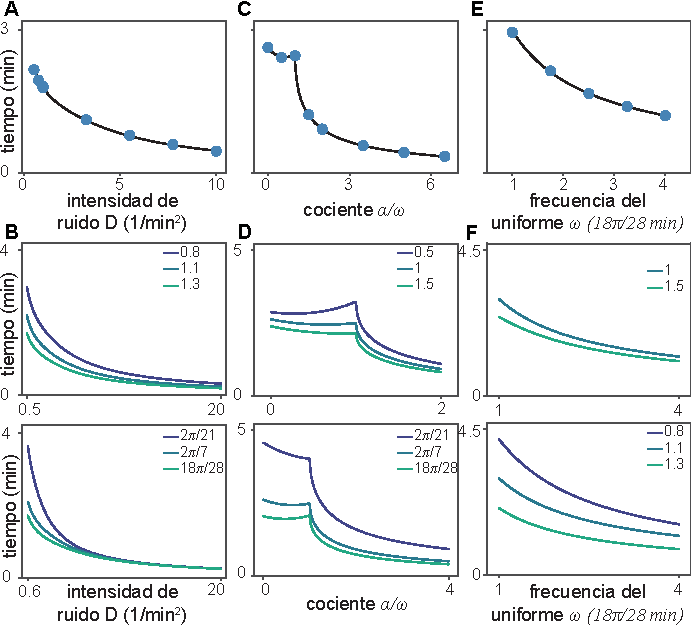
\includegraphics[width=1\columnwidth]{figures/chapter6/C6_duration.pdf} 
    \caption{\textbf{Duración de pulsos del modelo de fase con bifurcación de ciclo infinito y ruido blanco gaussiano aditivo.} (A,B) Duración de pulsos $T_\xi$ en función de la intensidad de ruido $D$. En B el cociente adimensional \dddelta (arriba) y la frecuencia del uniforme (abajo, en $1/\text{min}$) se encuentran codificados en escala de colores. (C,D) Duración de pulsos $T_\xi$ en función de el cociente adimensional \dddelta. En D la intensidad de ruido (arriba, en $1/\text{min}^2$) y la frecuencia del uniforme (abajo, en $1/\text{min}$) se encuentran codificados en escala de colores. (E,F) Duración de pulsos $T_\xi$ en función de la frecuencia del uniforme $\omega$. En F la intensidad de ruido (arriba, en $1/\text{min}^2$) y la frecuencia del uniforme (abajo, en $1/\text{min}$) se encuentran codificados en escala de colores (A-F). $\omega = 18\pi/28 \;\text{min}^{-1}$, $\dddelta = 1.1$ , y $D = 1 \;\text{min}^{-2}$, a excepción de que se especifique otro valor. (A,C,E)  Los puntos azules indican los resultados de los cálculos numéricos, y la línea negra indica el resultado de la expresión analítica \ref{C6_eq:Txi}. Las simulaciones numéricas fueron $N=10^6$, con un paso $dt = 10^{-5}$ y una frecuencia de adquisición de $d=1$.}
    \label{C6_fig:duration}
\end{figure}


En resumen, logramos obtener una expresión para la duración de pulsos del modelo de fase de bifurcación de ciclo infinito y ruido blanco gaussiano aditivo. Observamos analíticamente y con simulaciones computacionales que la duración de pulsos depende del ruido tanto en el caso excitable como en el oscilatorio. Esta dependencia es uniforme, y menores duraciones se consiguen con mayores valores de intensidad de ruido. Este comportamiento es coherente con la disminución de duraciones de pulsos con el aumento de la perturbación que obtuvimos para el caso excitable del modelo determinista. Además, hayamos que la duración de pulsos es finita en el punto de bifurcación donde $\dddelta = 1$, característica que tiene origen en añadir ruido blanco al modelo determinista. También hayamos que para valores de ruido y frecuencia del uniforme fijos, variar $\alpha$ en un entorno de la bifurcación puede eventualmente conducir a oscilaciones en el régimen oscilatorio, y actividad pulsátil en el régimen excitable, con duraciones de pulso similares. Este resultado sugiere que existen parámetros para los cuales en transiciones entre el régimen oscilatorio y el excitable generadas a través de variaciones en la amplitud de modulación la duración de pulsos media podría conservarse. 


\section{Conclusiones y discusión}

En los capítulos anteriores mostramos evidencia que favorece la hipótesis de que la dinámica de activación de ERK consiste en oscilaciones intermitentes, con transiciones entre intervalos de silencio, oscilatorios y pulsos aislados. Creemos que las oscilaciones están controladas por la dosis de FGF4, que además controla cuánto duran los intervalos oscilatorios. Tanto la duración de pulsos como el intervalo de interpulsado poseen valores modales similares, que parecen conservarse ante distintas dosis de estímulo extracelular. Aspiramos formalizar estas ideas en un modelo matemático de baja dimensionalidad. En este capítulo introdujimos los bloques teóricos fundamentales a partir de los cuales buscamos establecer un diálogo entre la teoría y los experimentos. A través de este diálogo esperamos construir una descripción teórica que recapitule las principales características de las oscilaciones intermitentes de la dinámica de activación de ERK que observamos en los experimentos. 


%modelo determinista
En la primera parte de este capítulo, mostramos los aspectos salientes de un modelo capaz de reproducir los distintos elementos dinámicos que observamos en las oscilaciones intermitentes incorporando paulatinamente cada uno de sus ingredientes a partir de revisar e integrar resultados presentes en la bibliografía. Como la relación entre la amplitud de la señal adquirida del sensor de traslocación y la actividad dinámica de ERK es desconocida, no fue posible caracterizar la amplitud de las series temporales de actividad de ERK a partir de nuestros experimentos, y decidimos no incorporar este aspecto en la teoría por el momento. Elegimos describir el estado dinámico del sistema con una variable angular o fase, e interpretamos como pulsos de ERK a los ciclos de la fase, y la señal de actividad según la ecuación \ref{C5_eq:seno_fase}. 

%modelo determinista
Comenzamos por presentar un modelo de fase con bifurcación de ciclo infinito con sólo dos parámetros: la frecuencia del caso uniforme y la amplitud de modulación (ecuación \ref{C5_eq:adler_determinista}). Vimos que con este modelo es posible obtener oscilaciones y silencios variando el cociente de los parámetros del modelo para atravesar la bifurcación. De un lado de la bifurcación, el régimen oscilatorio es no-uniforme (figura \ref{C5_fig:adler_determinista_oscilatorio}), y la no-uniformidad está regulada por la amplitud de modulación. Cuando se atraviesa la bifurcación, aparecen un punto fijo inestable y un punto fijo estable. El sistema tiende a permanecer en el punto fijo estable en su estado estacionario (figura \ref{C5_fig:adler_determinista_excitable}), lo que conduce a silencios en la señal. 

%excitabilidad
Observamos que, en el régimen que da lugar a silencios, es posible generar actividad pulsátil excitando al sistema dinámico. Cuando se le aplica una perturbación mayor al umbral de excitabilidad, la fase sobrepasa el punto fijo inestable y realiza una excursión antes de regresar al punto fijo estable. Con esto, la fase presenta un ciclo y la señal, un pulso. El umbral de excitabilidad es la distancia angular entre los puntos fijos, que está regulada por el cociente de los parámetros del modelo. Es posible que estos pulsos aparezcan entre silencios, por lo que parecen ser buenos candidatos para reproducir los pulsos aislados de la señal de actividad de ERK. A partir de esta idea, proponemos incorporar al modelo teórico la posibilidad de tener perturbaciones de manera sistemática a partir de agregar ruido blanco gaussiano aditivo al modelo de fase de bifurcación de ciclo infinito \cite{Lindner2004} (ecuación \ref{C6_eq:adler_white_noise}).


%efecto del ruido en el modelo
Observamos que el ruido promueve las excursiones del sistema dinámico a lo largo de la circunferencia trigonométrica, que en la señal se traduce en actividad pulsátil en el régimen excitable (figura \ref{C6_fig:traces}). A partir de analizar espectro de consenso de la señal y el correspondiente factor de calidad, identificamos que existe un valor de intensidad del ruido que optimiza la coherencia de la actividad pulsátil en este régimen, efecto conocido como resonancia estocástica (figura \ref{C6_fig:SR}). Contrariamente a nuestra intuición, ante determinadas circunstancias el ruido puede mejorar el rendimiento de determinados procesos. Por ejemplo, la resonancia estocástica puede optimizar la transmisión de información \cite{Gammaitoni1998}. Por otro lado, en el régimen oscilatorio observamos que las oscilaciones pierden su regularidad a medida que crece el ruido, y el ruido destruye la coherencia de las oscilaciones (figuras \ref{C6_fig:traces}, \ref{C6_fig:SR}). 


%conclusion 
Con el modelo con ruido blanco gaussiano es posible generar los principales elementos dinámicos que caracterizamos en las oscilaciones intermitentes: intervalos oscilatorios, de silencio y pulsos aislados. A partir de esta característica, se abre la pregunta de si es posible explotar sus propiedades o combinar estos elementos dinámicos para lograr reproducir nuestras observaciones de la dinámica de actividad de ERK en un modelo con la menor cantidad de parámetros posible. Por ejemplo, ¿es posible reproducir las transiciones entre intervalos oscilatorios, silencios y pulsos aislados perturbando de manera sistemática al sistema en el régimen excitable?, ¿pueden las oscilaciones intermitentes ser descriptas como oscilaciones desordenadas?. Como alternativa, ¿pueden ser descriptas como transiciones entre el estado excitable y el oscilatorio? 


%motivación para la duración de pulsos
Analizar cómo depende la duración de pulsos de los parámetros del modelo con el que proponemos comenzar a trabajar contribuye a evaluar posibles descripciones de las oscilaciones intermitentes. Estudiamos cómo se comporta la duración de pulsos ante la variación de los parámetros del modelo, a partir de analizar su expresión analítica. Comenzamos por analizar este comportamiento en el modelo determinista. 



%duración de pulsos modelo determinista  
Dedujimos la expresión analítica de la duración de pulsos en el régimen oscilatorio del modelo determinista \cite{Strogatz1994} (ecuación \ref{C5_eq:T_osc}). Para obtener una expresión analítica de la duración de pulsos en el régimen excitable, definimos un pulso cuando el sistema sobrepasa el punto fijo inestable y realiza una excursión hacia el punto fijo estable siguiente, y la duración de un pulso como el tiempo que tarda el sistema en llegar al punto fijo estable, habiendo partido del inestable (ecuación \ref{C5_eq:T_exc_def}, figura \ref{C5_fig:T_exc_def}). Para representar una perturbación que de lugar a un pulso, realizamos la integral en un entorno de los puntos fijos (ecuación \ref{C5_eq:T_exc_def_eps}, figura \ref{C5_fig:T_exc_def}). Calculamos la expresión analítica de la duración de pulsos para el régimen excitable (expresión \ref{C5_eq:T_exc}, figura \ref{C5_fig:T_exc_res}), cuyo comportamiento está en acuerdo con mediciones numéricas. En este caso, la duración de pulsos es el producto de dos factores: una expresión análoga a la duración de pulsos para el régimen oscilatorio, y un factor que depende del cociente de los parámetros del modelo y de la medida del entorno de los puntos fijos que usamos para integrar (expresión \ref{C5_eq:T_exc_aprox}).


%resultados
Nuestros resultados muestran que la duración de pulsos depende de la relación entre la amplitud de modulación y la frecuencia del uniforme en el modelo determinista. En el entorno entorno de la bifurcación la duración de pulsos varía fuertemente, y en la bifurcación diverge. Esto sugiere que ésta variaría en caso de tener transiciones entre el régimen oscilatorio y el excitable generadas a través de variaciones en la amplitud de modulación. Además, en el régimen excitable la duración de pulsos también depende de la magnitud de la perturbación, donde perturbaciones más grandes dan lugar a duraciones más pequeñas, y 
perturbaciones pequeñas conducen a duración de pulsos divergentes. 

%duracion de pulsos en ruido blanco
Para estudiar cómo el ruido regulariza estas divergencias, calculamos la duración de pulsos en el modelo con ruido blanco. Definimos a la duración de pulsos media como el tiempo medio que tarda el sistema en alcanzar el punto fijo estable, dado que el comenzó en el punto fijo inestable y durante ese tiempo no volvió al punto fijo inestable. Para calcularla, resolvimos un problema de tiempo de primer pasaje y utilizamos el formalismo de Laplace (figura \ref{C6_fig:duration}). Hicimos extensivo este cálculo al caso oscilatorio, y nuestros resultados fueron consistentes con mediciones numéricas. 

%resultados
Observamos que la duración de pulsos depende del ruido tanto en el caso excitable como en el oscilatorio. Esta dependencia es uniforme, y menores duraciones se consiguen con mayores valores de intensidad de ruido. Este comportamiento es coherente con la disminución de duraciones de pulsos con el aumento de la perturbación que obtuvimos para el caso excitable del modelo determinista. Además, hayamos que la duración de pulsos es finita en el punto de bifurcación, característica que tiene origen en añadir ruido blanco al modelo determinista. Observamos que a medida que el ruido disminuye, la duración de pulsos en la bifurcación es cada vez más grande, posiblemente tendiendo al resultado determinista. También hayamos que para valores de ruido y frecuencia del uniforme fijos, variar la amplitud de modulación en un entorno de la bifurcación puede eventualmente conducir a oscilaciones en el régimen oscilatorio, y actividad pulsátil en el régimen excitable, con duraciones de pulso similares. Este resultado sugiere que existen parámetros para los cuales en transiciones entre el régimen oscilatorio y el excitable generadas a través de variaciones en la amplitud de modulación la duración de pulsos media podría conservarse. Alternativamente, pequeñas variaciones de los parámetros cerca de la bifurcación podrían dar lugar a variabilidad en la duración de pulsos consistentes con el ancho de las distribuciones de duración de pulsos que observamos en los experimentos. Además, la variabilidad que posiblemente aporte el carácter estocástico de las perturbaciones del modelo que proponemos también podría aportar a reproducir este aspecto de nuestras observaciones. 

%un chamullo sobre ruido
En sistemas lejos del equilibrio, el ruido está presente inevitablemente, y sus orígenes pueden ser muy diversos \cite{Lindner2004}. En particular, el ruido puede estar presente en sistemas excitables como reacciones químicas, lásers, la dinámica del clima, neuronas, e incluso en redes de transducción de señales intracelulares como las que regulan la dinámica de ERK es ESCs. Cómo el ruido afecta a sistemas excitables es una pregunta relevante para muchas áreas del conocimiento, y presenta muchas aplicaciones.


%importancia modelo teórico
La vía de señalización de ERK regula múltiples funciones celulares en diversos tipos de células. Los principales mecanismos implicados en la activación de la vía ERK han sido bien caracterizados, y su regulación es altamente compleja (capítulo \ref{ch1}). Un modelo que contemple los componentes e interacciones de esta red resulta interesante, y ayudaría a entender cuál es origen de la dinámica de activación de ERK y las oscilaciones intermitentes. Por otro lado, desarrollar una descripción de baja dimensionalidad de la dinámica de activación de ERK en ESCs nos daría información para comprender cuál es el mecanismo dinámico que promueve esta activación. Además, nos permitiría entender cuáles son las propiedades dinámicas propias del tipo celular, y cuáles de estas características codifican información relevante para tomar decisiones de destino celular. Asimismo, una descripción de baja dimensionalidad de la dinámica de activación de ERK en ESCs es interesante desde el enfoque puramente teórico. La activación de ERK representa un tipo de dinámica previamente no descripta, y desarrollar una descripción teórica así como entender sus principales propiedades dinámicas es un aporte interesante. 

\end{document}


En principio, esta caracterización es compatible con que haya un conjunto de parámetros que den origen a una duración de pulsos como en la que observamos en los experimentos. En lo próximo, evaluamos concretamente la posibilidad de que el modelo teórico propuesto pueda reproducir la estadística de nuestras mediciones experimentales, para luego calibrarlo y entender qué características de las oscilaciones intermitentes de actividad de ERK es capaz de reproducir. 



